%%%%%%%%%%%%%%%%%%%%%%%%%%%%%%%%%%%%%%%%%
% Beamer Presentation
% LaTeX Template
% Version 1.0 (10/11/12)
%
% This template has been downloaded from:
% http://www.LaTeXTemplates.com
%
% License:
% CC BY-NC-SA 3.0 (http://creativecommons.org/licenses/by-nc-sa/3.0/)
%
%%%%%%%%%%%%%%%%%%%%%%%%%%%%%%%%%%%%%%%%%

%----------------------------------------------------------------------------------------
%    PACKAGES AND THEMES
%----------------------------------------------------------------------------------------

\documentclass{beamer}
\usepackage{animate}
\usepackage{float}
\usepackage{bm}
\usepackage{mathtools}

\newcommand{\ChoL}{\mathsf{L}}
\newcommand{\bx}{\mathbf{x}}
\newcommand{\ii}{\mathrm{i}}
\newcommand{\bxi}{\bm{\xi}}
\newcommand{\bmu}{\bm{\mu}}
\newcommand{\bb}{\mathbf{b}}
\newcommand{\bA}{\mathbf{A}}
\newcommand{\bJ}{\mathbf{J}}
\newcommand{\bB}{\mathbf{B}}
\newcommand{\bM}{\mathbf{M}}

\newcommand{\by}{\mathbf{y}}
\newcommand{\bw}{\mathbf{w}}

\newcommand{\bX}{\mathbf{X}}
\newcommand{\bY}{\mathbf{Y}}
\newcommand{\bs}{\mathbf{s}}
\newcommand{\sign}{\mathrm{sign}}
\newcommand{\bt}[0]{\bm{\theta}}
\newcommand{\bc}{\mathbf{c}}
\newcommand{\bzero}{\mathbf{0}}
\renewcommand{\bf}{\mathbf{f}}
\newcommand{\bu}{\mathbf{u}}
\newcommand{\bv}[0]{\mathbf{v}}
\mode<presentation> {

% The Beamer class comes with a number of default slide themes
% which change the colors and layouts of slides. Below this is a list
% of all the themes, uncomment each in turn to see what they look like.

%\usetheme{default}
%\usetheme{AnnArbor}
%\usetheme{Antibes}
%\usetheme{Bergen}
%\usetheme{Berkeley}
%\usetheme{Berlin}
%\usetheme{Boadilla}
%\usetheme{CambridgeUS}
%\usetheme{Copenhagen}
%\usetheme{Darmstadt}
%\usetheme{Dresden}
%\usetheme{Frankfurt}
%\usetheme{Goettingen}
%\usetheme{Hannover}
%\usetheme{Ilmenau}
%\usetheme{JuanLesPins}
%\usetheme{Luebeck}
\usetheme{Madrid}
%\usetheme{Malmoe}
%\usetheme{Marburg}
%\usetheme{Montpellier}
%\usetheme{PaloAlto}
%\usetheme{Pittsburgh}
%\usetheme{Rochester}
%\usetheme{Singapore}
%\usetheme{Szeged}
%\usetheme{Warsaw}


% As well as themes, the Beamer class has a number of color themes
% for any slide theme. Uncomment each of these in turn to see how it
% changes the colors of your current slide theme.

%\usecolortheme{albatross}
\usecolortheme{beaver}
%\usecolortheme{beetle}
%\usecolortheme{crane}
%\usecolortheme{dolphin}
%\usecolortheme{dove}
%\usecolortheme{fly}
%\usecolortheme{lily}
%\usecolortheme{orchid}
%\usecolortheme{rose}
%\usecolortheme{seagull}
%\usecolortheme{seahorse}
%\usecolortheme{whale}
%\usecolortheme{wolverine}

%\setbeamertemplate{footline} % To remove the footer line in all slides uncomment this line
%\setbeamertemplate{footline}[page number] % To replace the footer line in all slides with a simple slide count uncomment this line

%\setbeamertemplate{navigation symbols}{} % To remove the navigation symbols from the bottom of all slides uncomment this line
}
\usepackage{booktabs}
\usepackage{makecell}
\usepackage{soul}
\newcommand{\red}[1]{\textcolor{red}{#1}}
%
%\usepackage{graphicx} % Allows including images
%\usepackage{booktabs} % Allows the use of \toprule, \midrule and \bottomrule in tables
%
%
%\usepackage{amsthm}
%
%\usepackage{todonotes}
%\usepackage{floatrow}
%
%\usepackage{pgfplots,algorithmic,algorithm}
%\usepackage[toc,page]{appendix}
%\usepackage{float}
%\usepackage{booktabs}
%\usepackage{bm}
%
%\theoremstyle{definition}
%
\newcommand{\RR}[0]{\mathbb{R}}
%
%\newcommand{\bx}{\mathbf{x}}
%\newcommand{\ii}{\mathrm{i}}
%\newcommand{\bxi}{\bm{\xi}}
%\newcommand{\bmu}{\bm{\mu}}
%\newcommand{\bb}{\mathbf{b}}
%\newcommand{\bA}{\mathbf{A}}
%\newcommand{\bJ}{\mathbf{J}}
%\newcommand{\bB}{\mathbf{B}}
%\newcommand{\bM}{\mathbf{M}}
%\newcommand{\bF}{\mathbf{F}}
%
%\newcommand{\by}{\mathbf{y}}
%\newcommand{\bw}{\mathbf{w}}
%\newcommand{\bn}{\mathbf{n}}
%
%\newcommand{\bX}{\mathbf{X}}
%\newcommand{\bY}{\mathbf{Y}}
%\newcommand{\bs}{\mathbf{s}}
%\newcommand{\sign}{\mathrm{sign}}
%\newcommand{\bt}[0]{\bm{\theta}}
%\newcommand{\bc}{\mathbf{c}}
%\newcommand{\bzero}{\mathbf{0}}
%\renewcommand{\bf}{\mathbf{f}}
%\newcommand{\bu}{\mathbf{u}}
%\newcommand{\bv}[0]{\mathbf{v}}

\AtBeginSection[]
{
   \begin{frame}
       \frametitle{Outline}
       \tableofcontents[currentsection]
   \end{frame}
}

%----------------------------------------------------------------------------------------
%    TITLE PAGE
%----------------------------------------------------------------------------------------
\usepackage{bm}
\newcommand*{\TakeFourierOrnament}[1]{{%
\fontencoding{U}\fontfamily{futs}\selectfont\char#1}}
\newcommand*{\danger}{\TakeFourierOrnament{66}}

\title[Physics Based Machine Learning]{Physics Based Machine Learning for Inverse Problems} % The short title appears at the bottom of every slide, the full title is only on the title page

\author[ADCME]{Kailai Xu and Eric Darve\\\quad\url{https://github.com/kailaix/ADCME.jl} \qquad      \\ $\star$ The Pathway to Physics Based Machine Learning $\star$} % Your name
%\institute[] % Your institution as it will appear on the bottom of every slide, may be shorthand to save space
%{
%%ICME, Stanford University \\ % Your institution for the title page
%%\medskip
%%\textit{kailaix@stanford.edu}\quad \textit{darve@stanford.edu} % Your email address
%}
\date{}% Date, can be changed to a custom date
% Mathematics of PDEs


\begin{document}

\usebackgroundtemplate{%
\begin{picture}(0,250)
\centering
	{{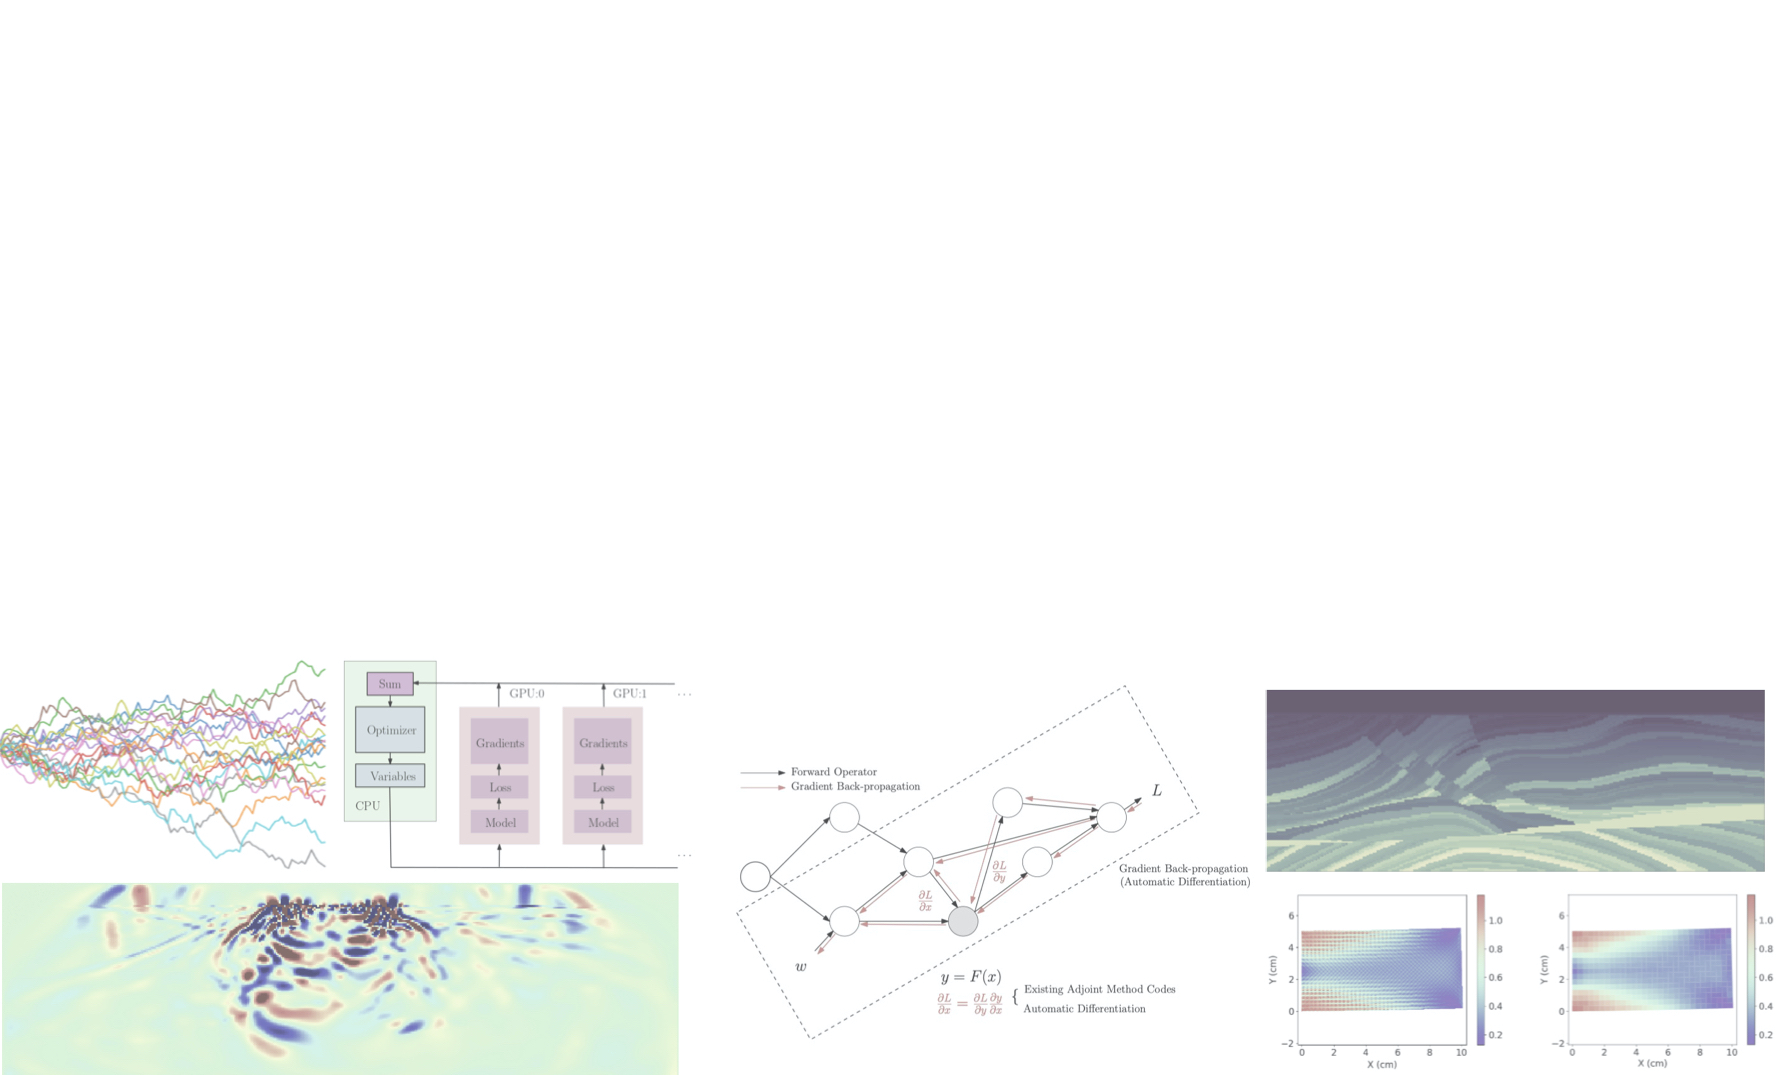
\includegraphics[width=1.0\paperwidth]{../background}}}
\end{picture}
  } 
%\usebackgroundtemplate{%
%  \includegraphics[width=\paperwidth,height=\paperheight]{figures/back}} 
\begin{frame}

\titlepage % Print the title page as the first slide

%dfa
\end{frame}
\usebackgroundtemplate{}

\section{Physics Based Machine Learning}



\begin{frame}
	\frametitle{Inverse Modeling}
	\begin{itemize}
		\item \textbf{Inverse modeling} identifies a certain set of parameters or functions with which the outputs of the forward analysis matches the desired result or measurement.
		\item Many real life engineering problems can be formulated as inverse modeling problems: shape optimization for improving the performance of structures, optimal control of fluid dynamic systems, etc.
		\begin{figure}[hbt]
  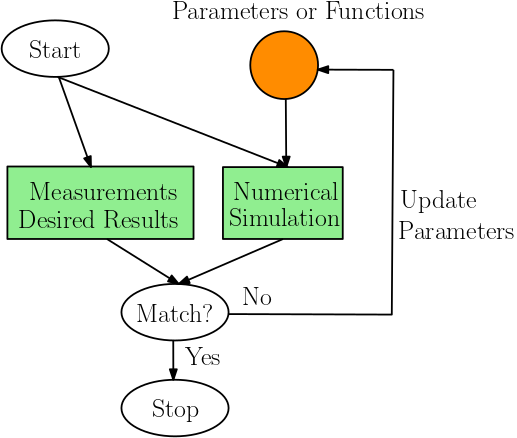
\includegraphics[width=0.4\textwidth]{../im.png}
  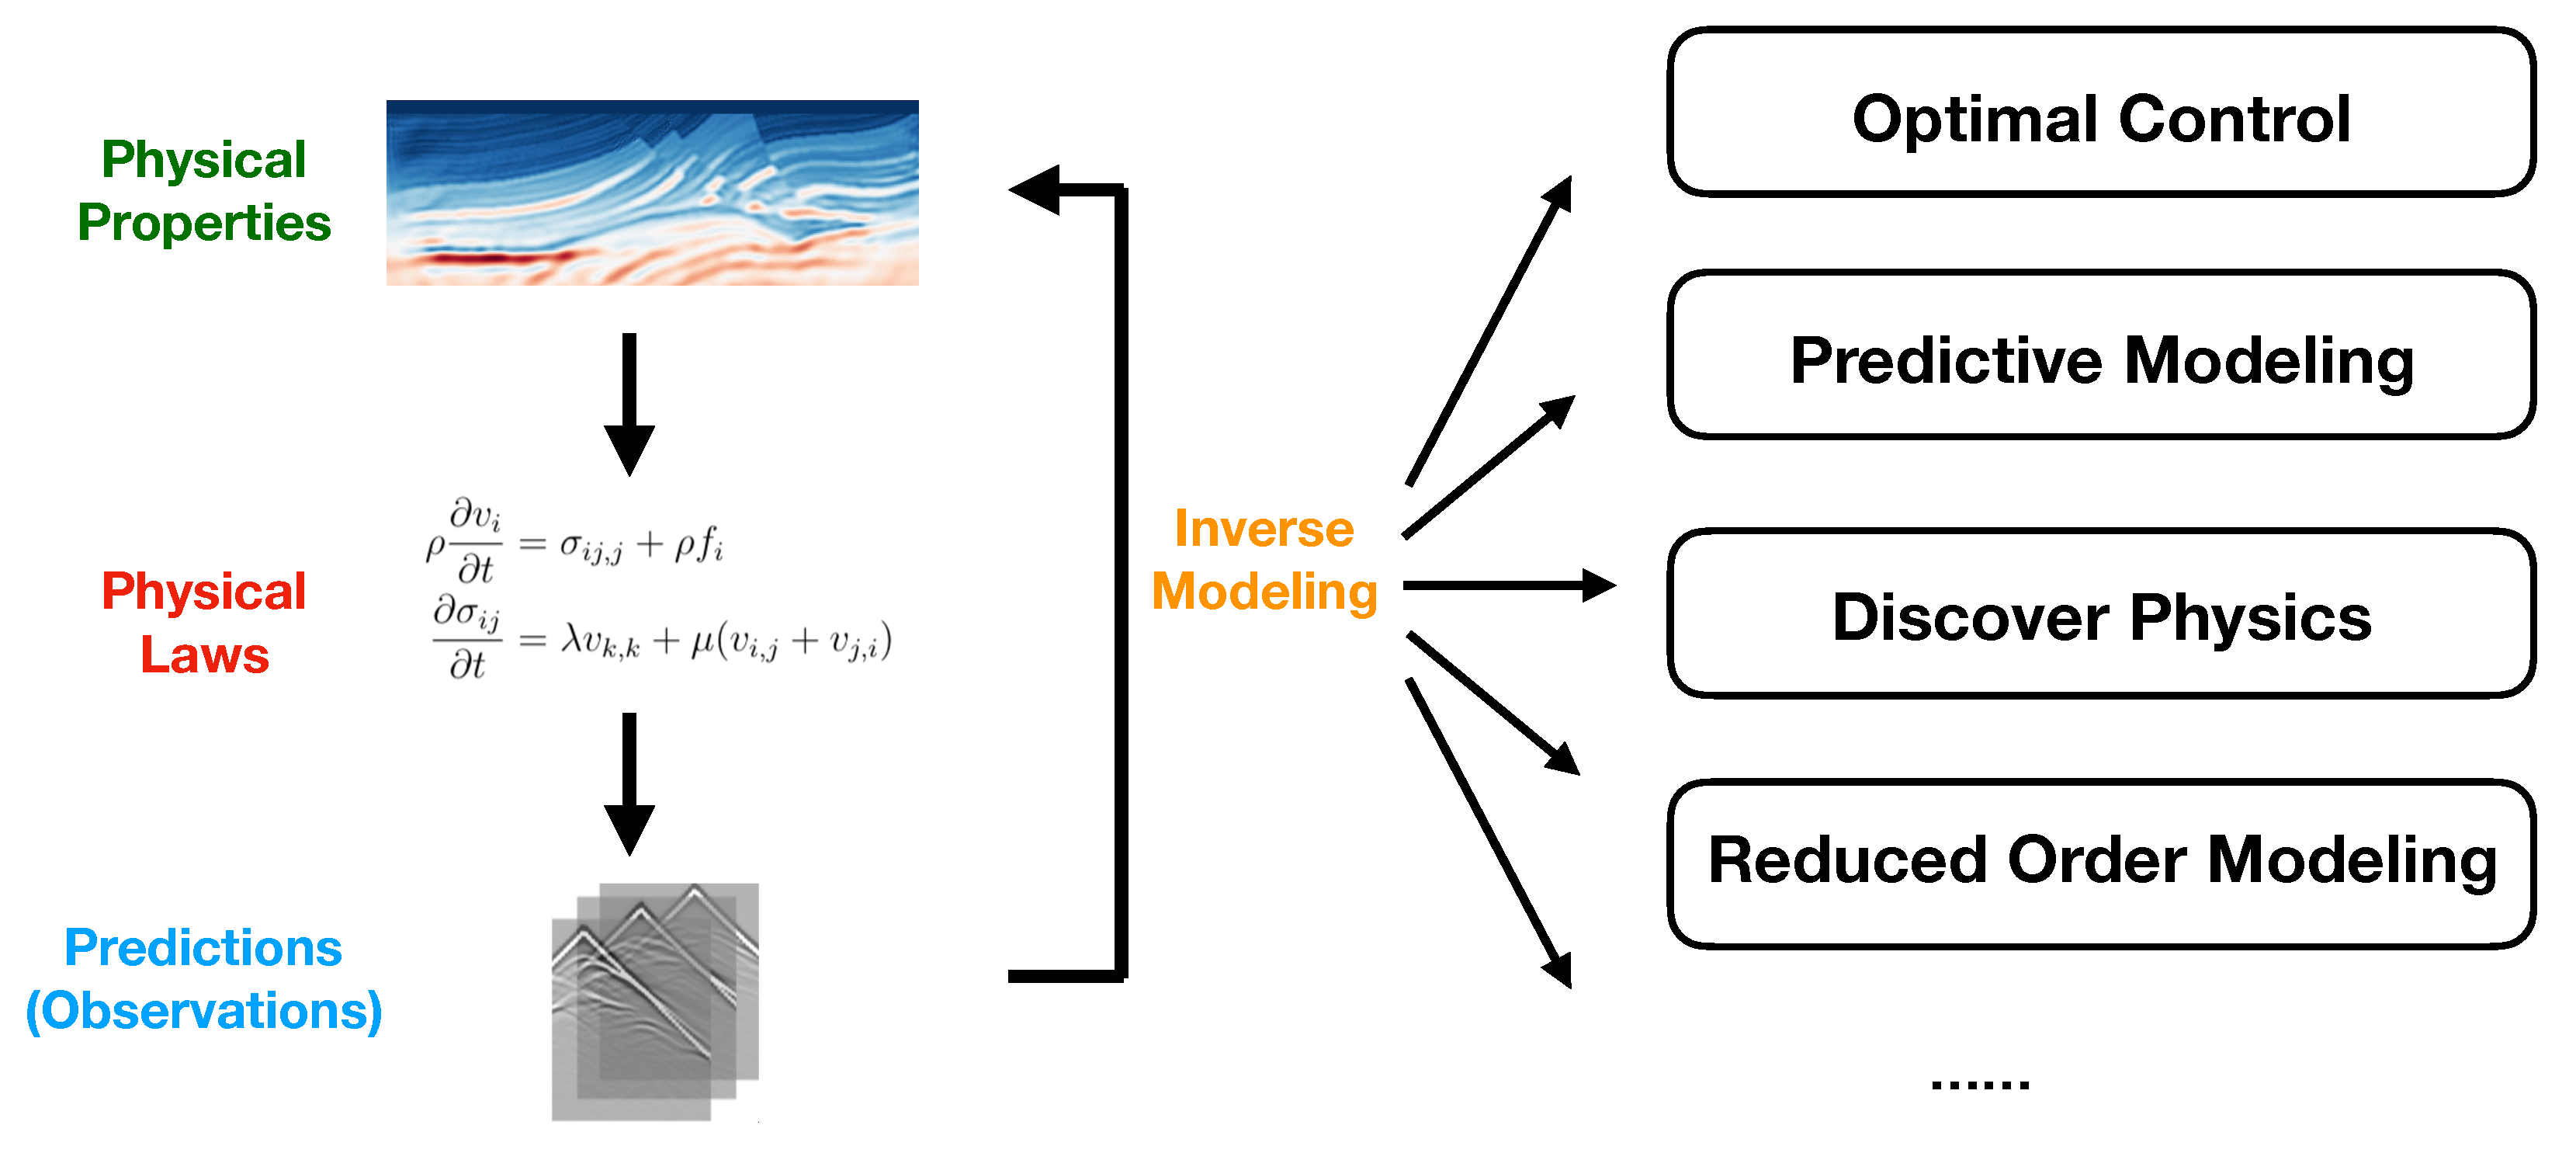
\includegraphics[width=0.45\textwidth]{../inverse2}
\end{figure}

	\end{itemize}
\end{frame}

\begin{frame}
	\frametitle{Physics Based Machine Learning}
	\begin{itemize}
		\item Classical physical modeling relies on efficient numerical schemes for discretizing conservation laws derived from first principles; deep learning learns statistical relations from large amounts of training data.
		\item We combine the best of the two worlds and invent \textbf{physics based machine learning}: \textcolor{red}{only the unknown is modeled with deep neural networks, and the known physical laws are solved with numerical schemes}.
	\end{itemize}
	\begin{figure}[hbt]
  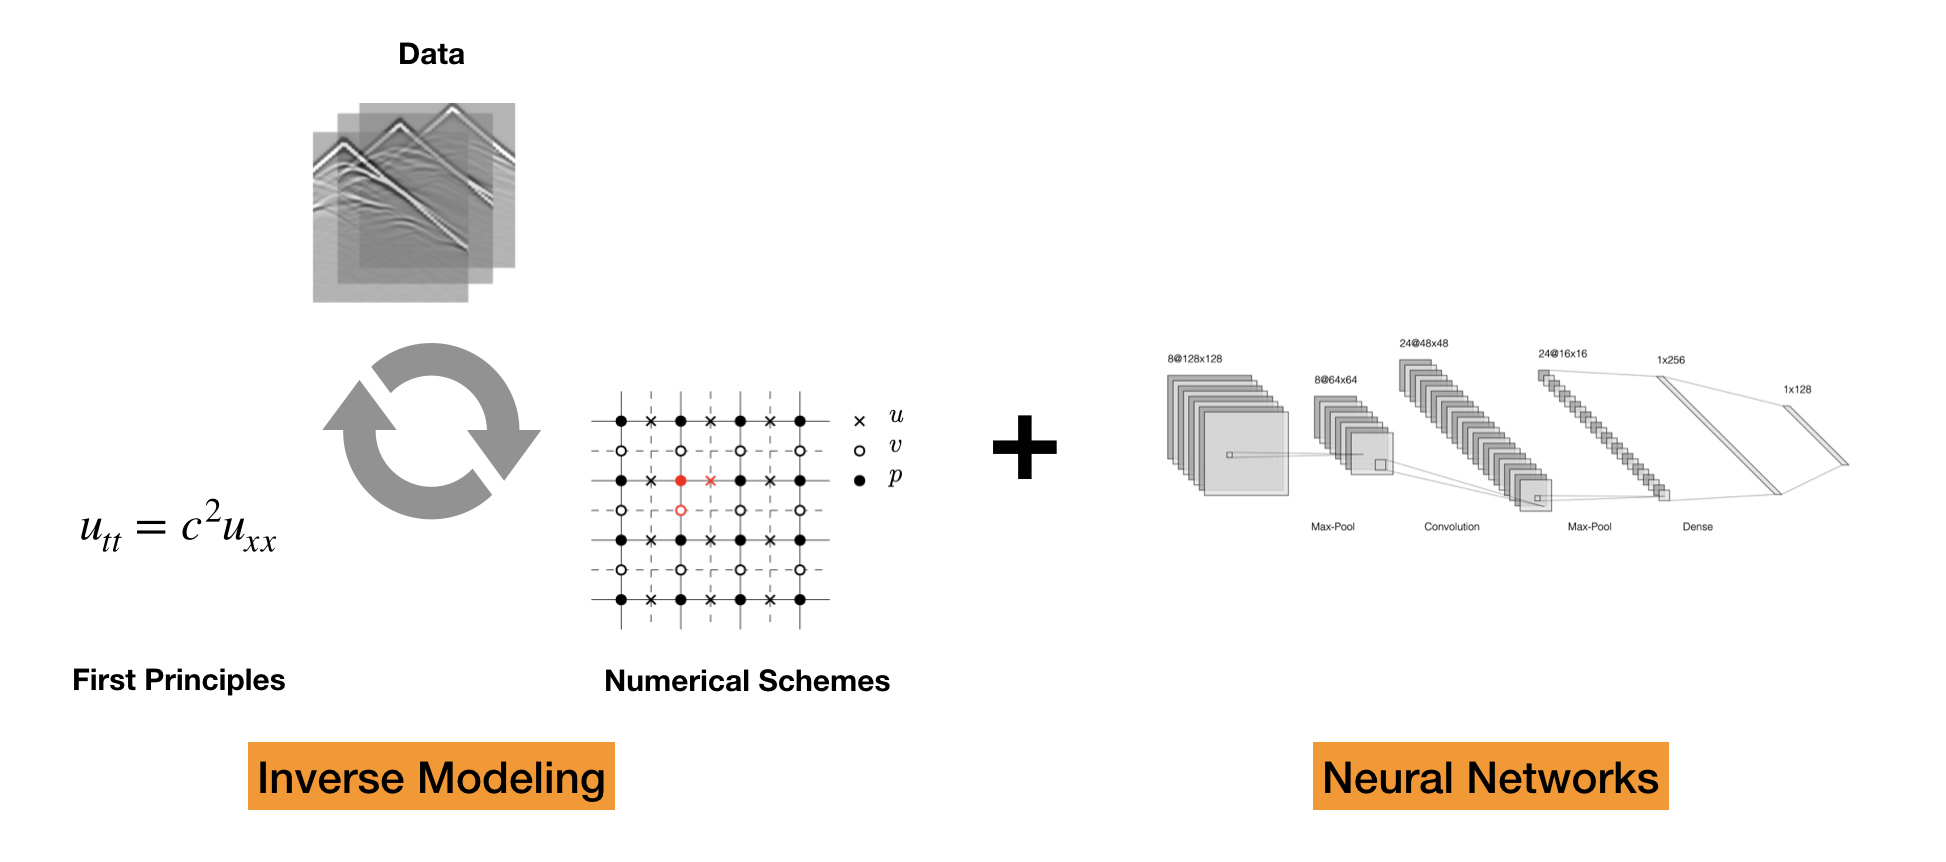
\includegraphics[width=0.75\textwidth]{../physics_based_machine_learning.png}
\end{figure}
\end{frame}

\section{Automatic Differentiation for Inverse Modeling}

\begin{frame}
	\frametitle{Automatic Differentiation}
The fact that bridges the \textcolor{red}{technical} gap between machine learning and inverse modeling:
	\begin{itemize}
		\item Deep learning (and many other machine learning techniques) and numerical schemes share the same computational model: composition of individual operators. 
	\end{itemize}
	

\begin{minipage}[t]{0.4\textwidth}

\



\begin{center}
	Back-propagation 

= 

 Automatic Differentiation 

=
 
 Adjoint-State Method
\end{center}
\end{minipage}~
\begin{minipage}[t]{0.6\textwidth}
\begin{figure}[hbt]
  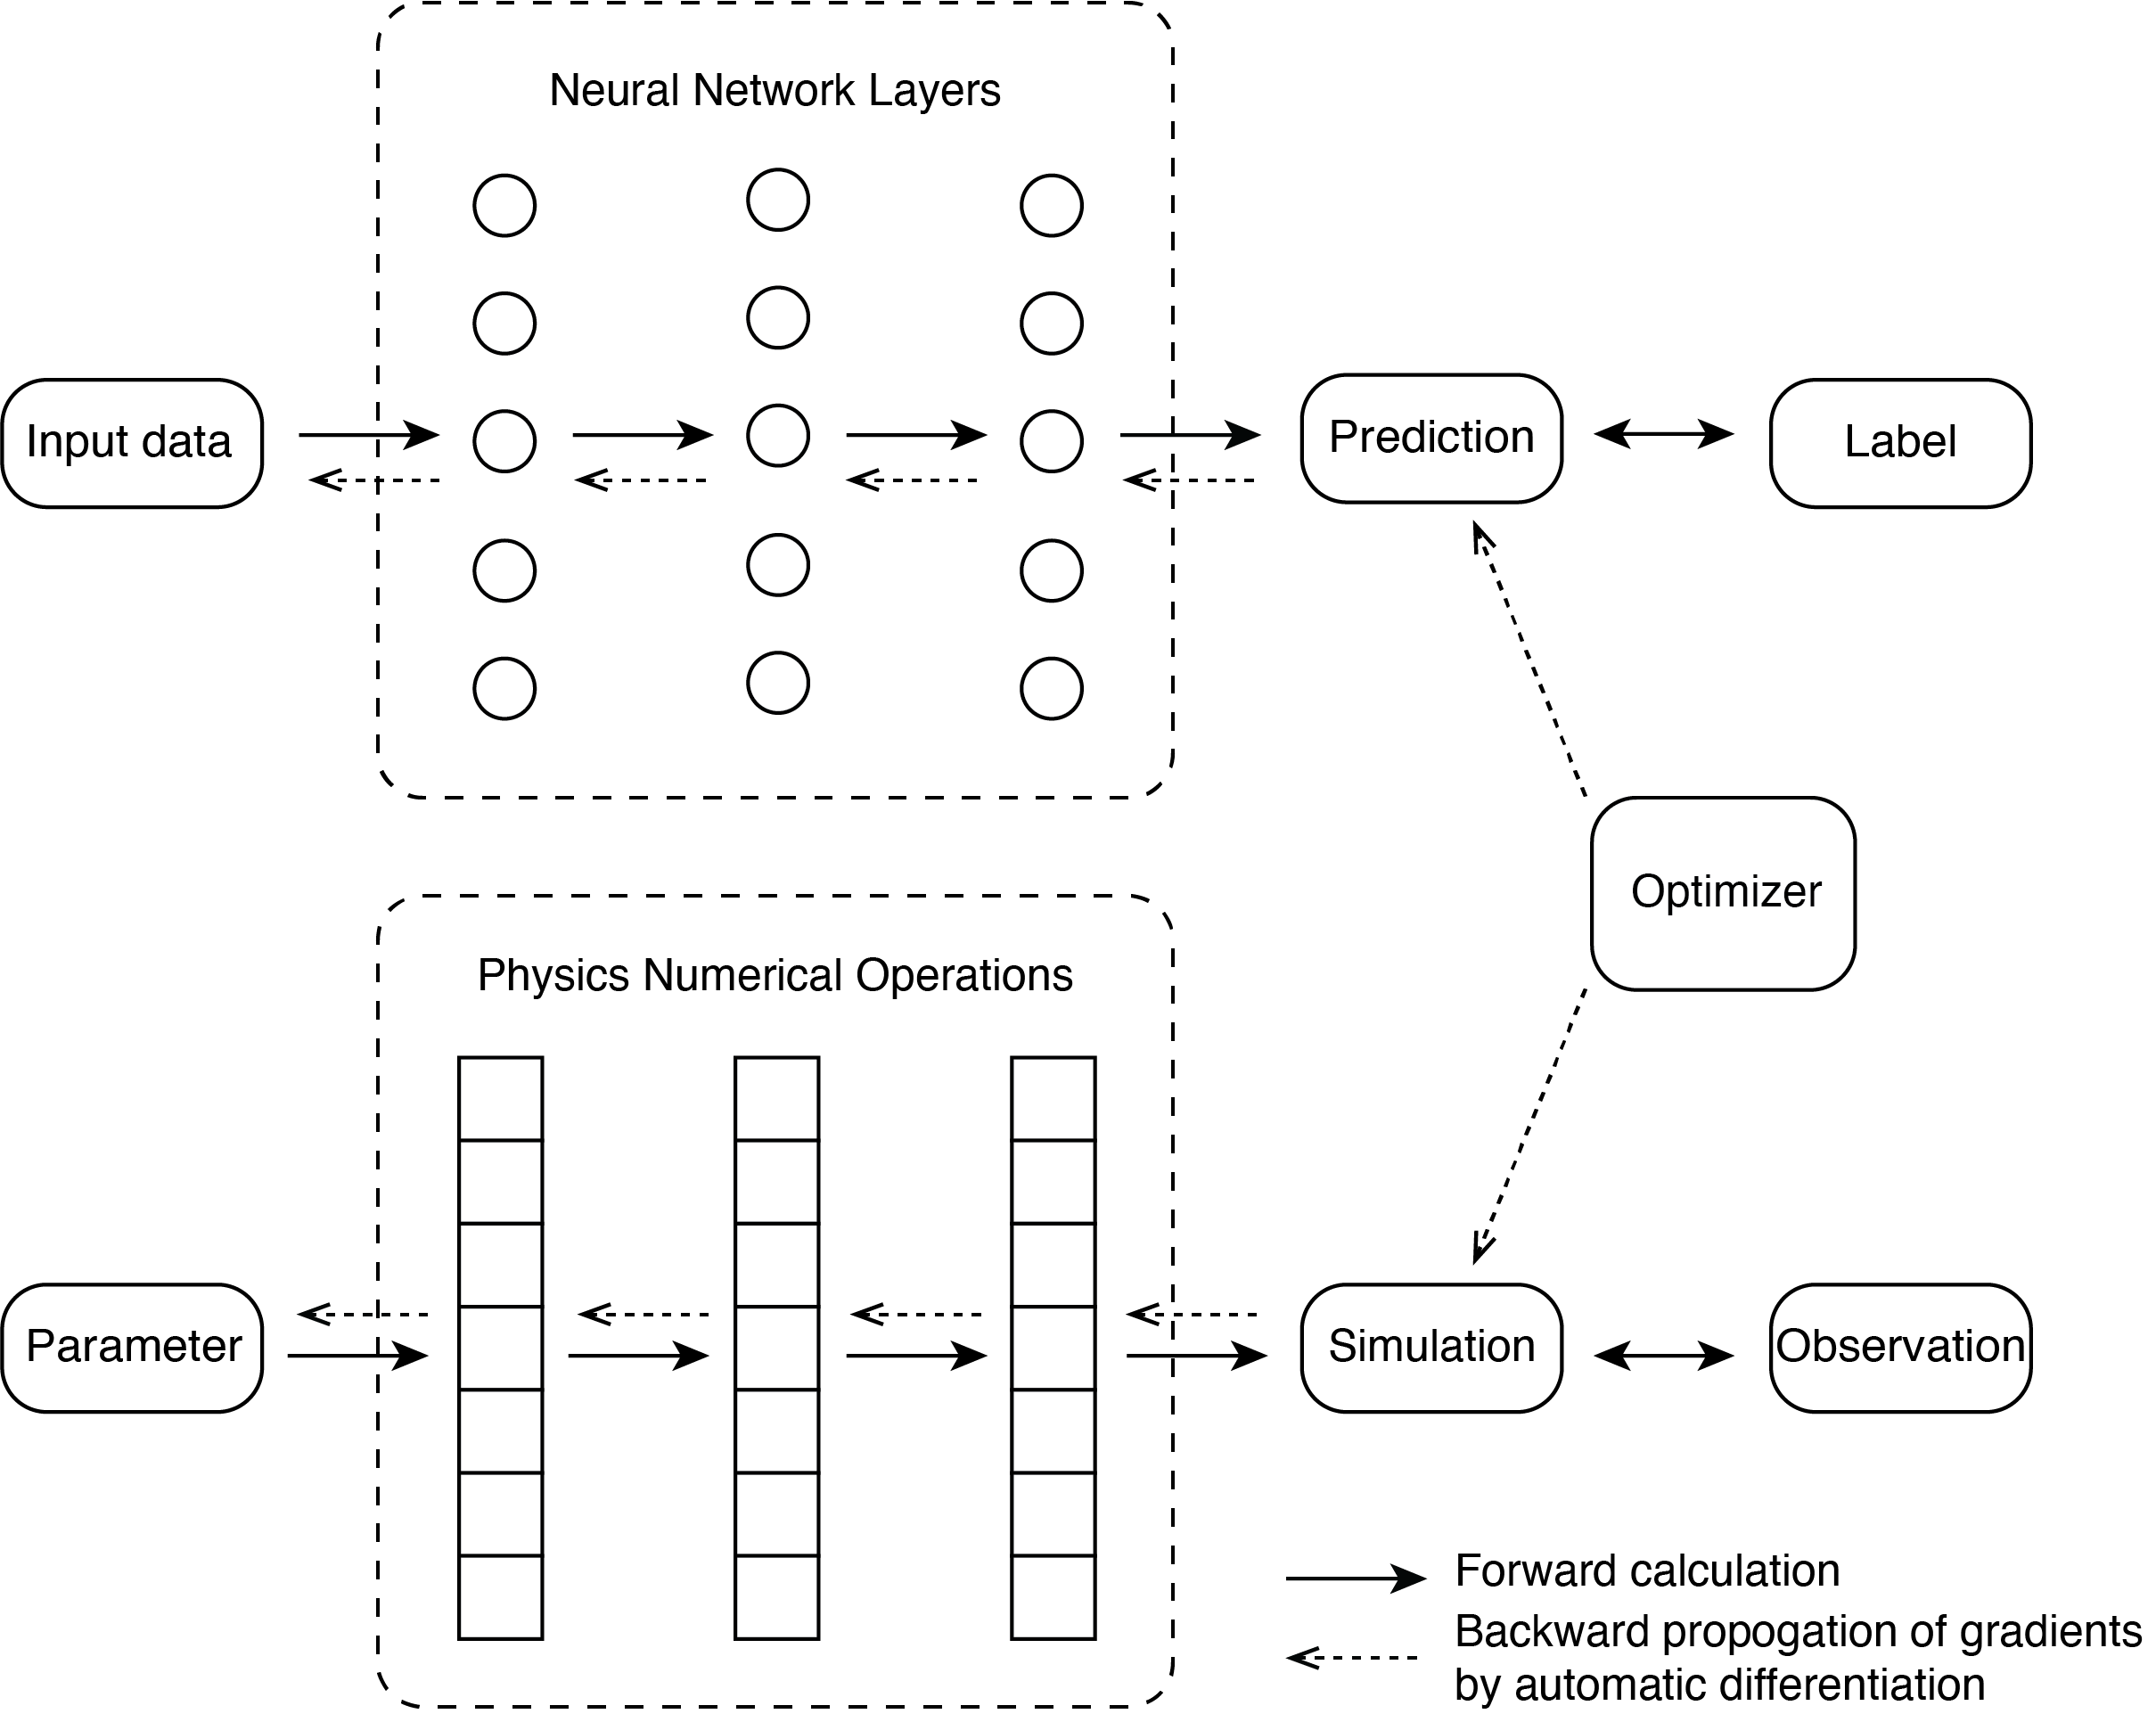
\includegraphics[width=0.8\textwidth]{../compare-NN-PDE.png}
\end{figure}
\end{minipage}

\end{frame}


\begin{frame}
	\frametitle{Automatic Differentiation: Computational Graph}
	
	\begin{itemize}
		\item A computational graph is a functional description of the required computation. In the computational graph, an edge represents \textcolor{red}{data}, such as a scalar, a vector, a matrix or a tensor. A node represents a \textcolor{red}{function (operator)} whose input arguments are the the incoming edges and output values are are the outcoming edges. 
		\item How to build a computational graph for $z = \sin(x_1+x_2) + x_2^2 x_3$?
	\end{itemize}
	
	\begin{figure}[hbt]
  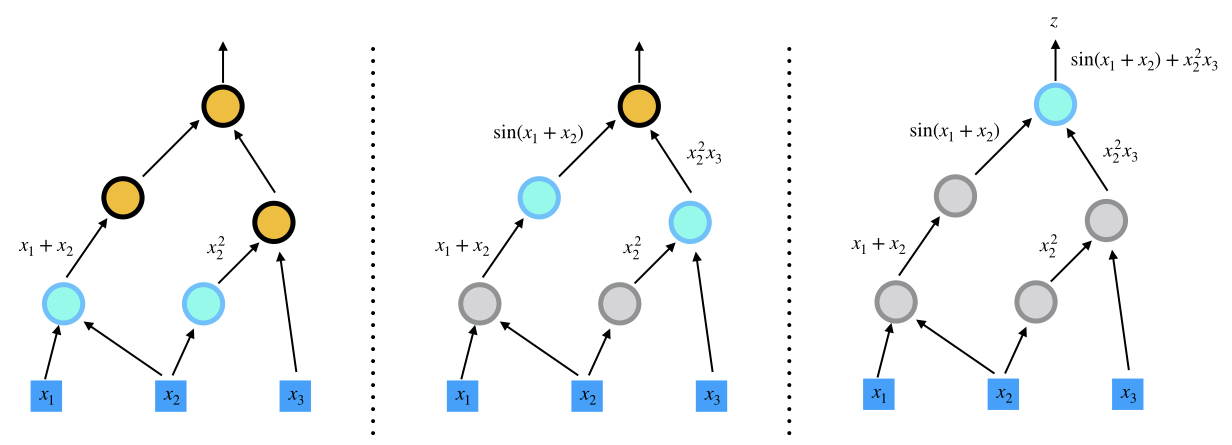
\includegraphics[width=1.0\textwidth]{../fd}
\end{figure}
\end{frame}

\begin{frame}
	\frametitle{Automatic Differentiation: Reverse-Mode}
	
	\begin{itemize}
		\item The reverse-mode automatic differentiation relies on the chain rule 
		$$\frac{\partial f\circ g (x)}{\partial x} = \frac{\partial f'\circ g(x)}{\partial g} \frac{\partial g'(x)}{\partial x}$$
		\item Let's see how to compute $\frac{\partial z}{\partial x_i}$, $i=1,2,3$ for $z = \sin(x_1+x_2) + x_2^2 x_3$
	\end{itemize}
	\centering
	\begin{figure}[hbt]
  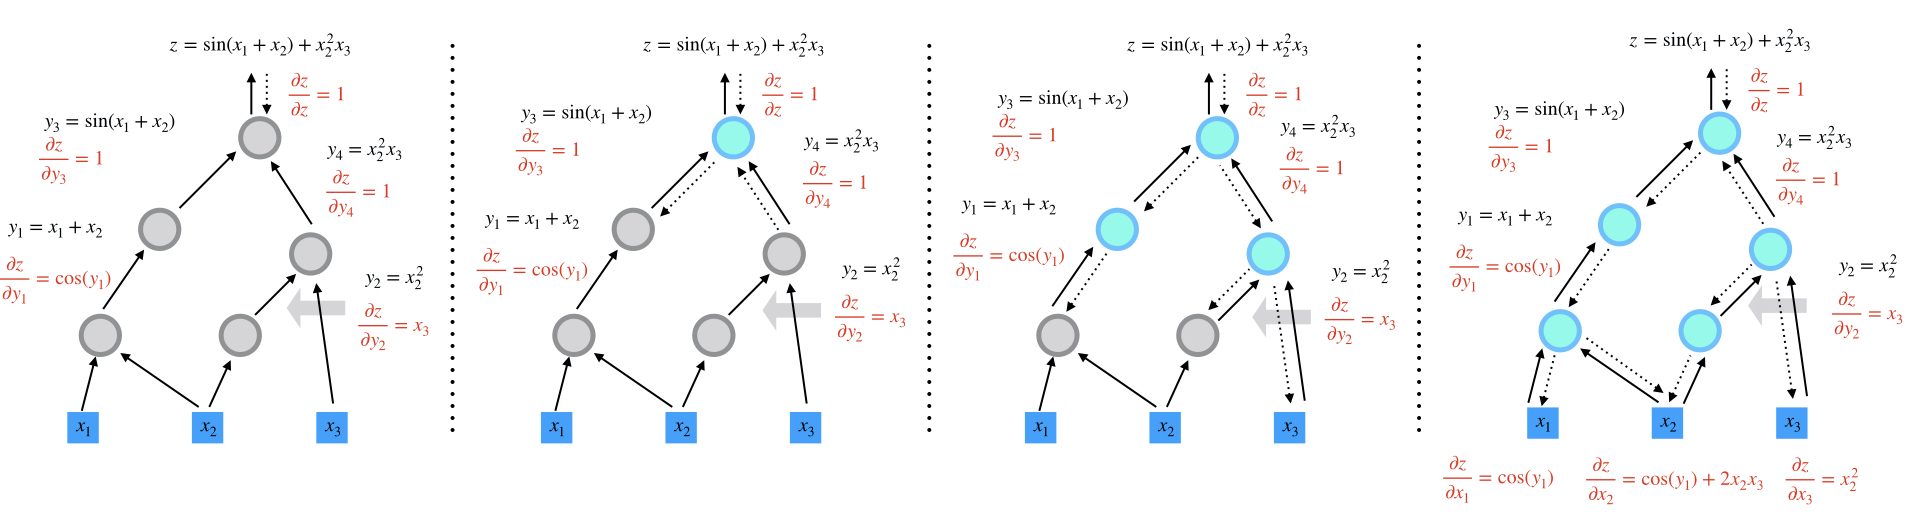
\includegraphics[width=1.0\textwidth]{../bd}
\end{figure}

\end{frame}

\begin{frame}
	\frametitle{Automatic Differentiation: Mathematical Description}
	\begin{minipage}[t]{0.49\textwidth}
	A computational graph starts from independent variables $x_1$, $x_2$, $\ldots$, $x_n$, which are transformed by the composition of operators $f_k$, $k = n+1, n+2, \ldots, N$
		$$\begin{aligned}
    x_{n+1} &= f_{n+1}(\mathbf{x}_{\pi({n+1})})\\
    x_{n+2} &= f_{n+2}(\mathbf{x}_{\pi({n+2})})\\
    \ldots\\
    x_{N} &= f_{N}(\mathbf{x}_{\pi({N})})\\
\end{aligned}$$
where $\pi(i) \in \{1,2,\ldots,i-1\}$. 
\end{minipage}~
\begin{minipage}[t]{0.49\textwidth}
  \begin{figure}[hbt]
  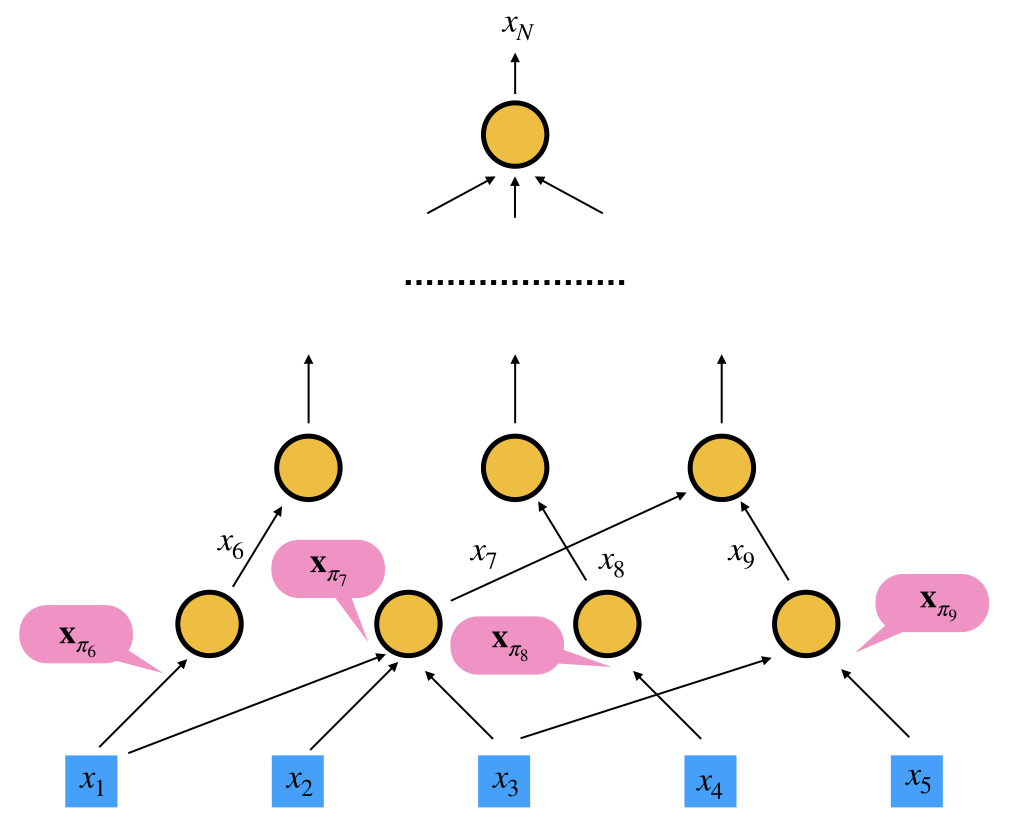
\includegraphics[width=1.0\textwidth]{../cg}
\end{figure}
\end{minipage}
\end{frame}

\begin{frame}
	\frametitle{Automatic Differentiation: Mathematical Description}
\begin{theorem}[Chain Rule]
	$$\frac{\partial x_N(x_1, x_2, \ldots, x_{i})}{\partial x_i} = \sum_{j\,:\,i\in \pi(j)}
    \frac{\partial x_N(x_1, x_2, \ldots, x_j)}{\partial x_j}
    \frac{\partial x_j(x_1, x_2, \ldots, x_{j-1})}{\partial x_i}$$
\end{theorem}
\begin{figure}[hbt]
  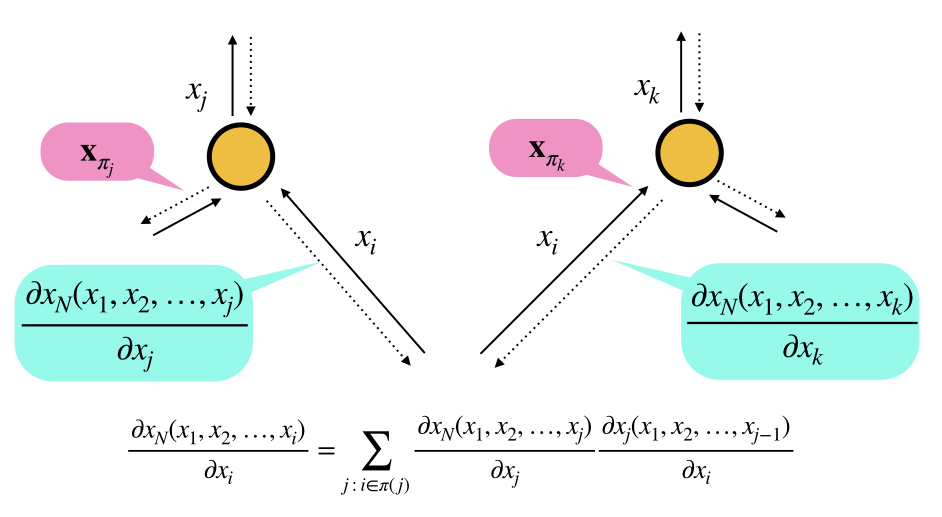
\includegraphics[width=0.6\textwidth]{../cg2}
\end{figure}
	
\end{frame}


\begin{frame}
	\frametitle{ADCME}
	\begin{itemize}
		\item ADCME allows users to use \textcolor{red}{high performance} and \textcolor{red}{mathematical friendly} programming language Julia to implement numerical schemes, and obtain the \textcolor{red}{comprehensive automatic differentiation functionality}, \textcolor{red}{heterogeneous computing capability}, \textcolor{red}{parallelism} and \textcolor{red}{scalability} provided by the TensorFlow backend. 
		\item ADCME simplifies programming and improves performance. 
	\end{itemize}
	\begin{figure}[hbt]
  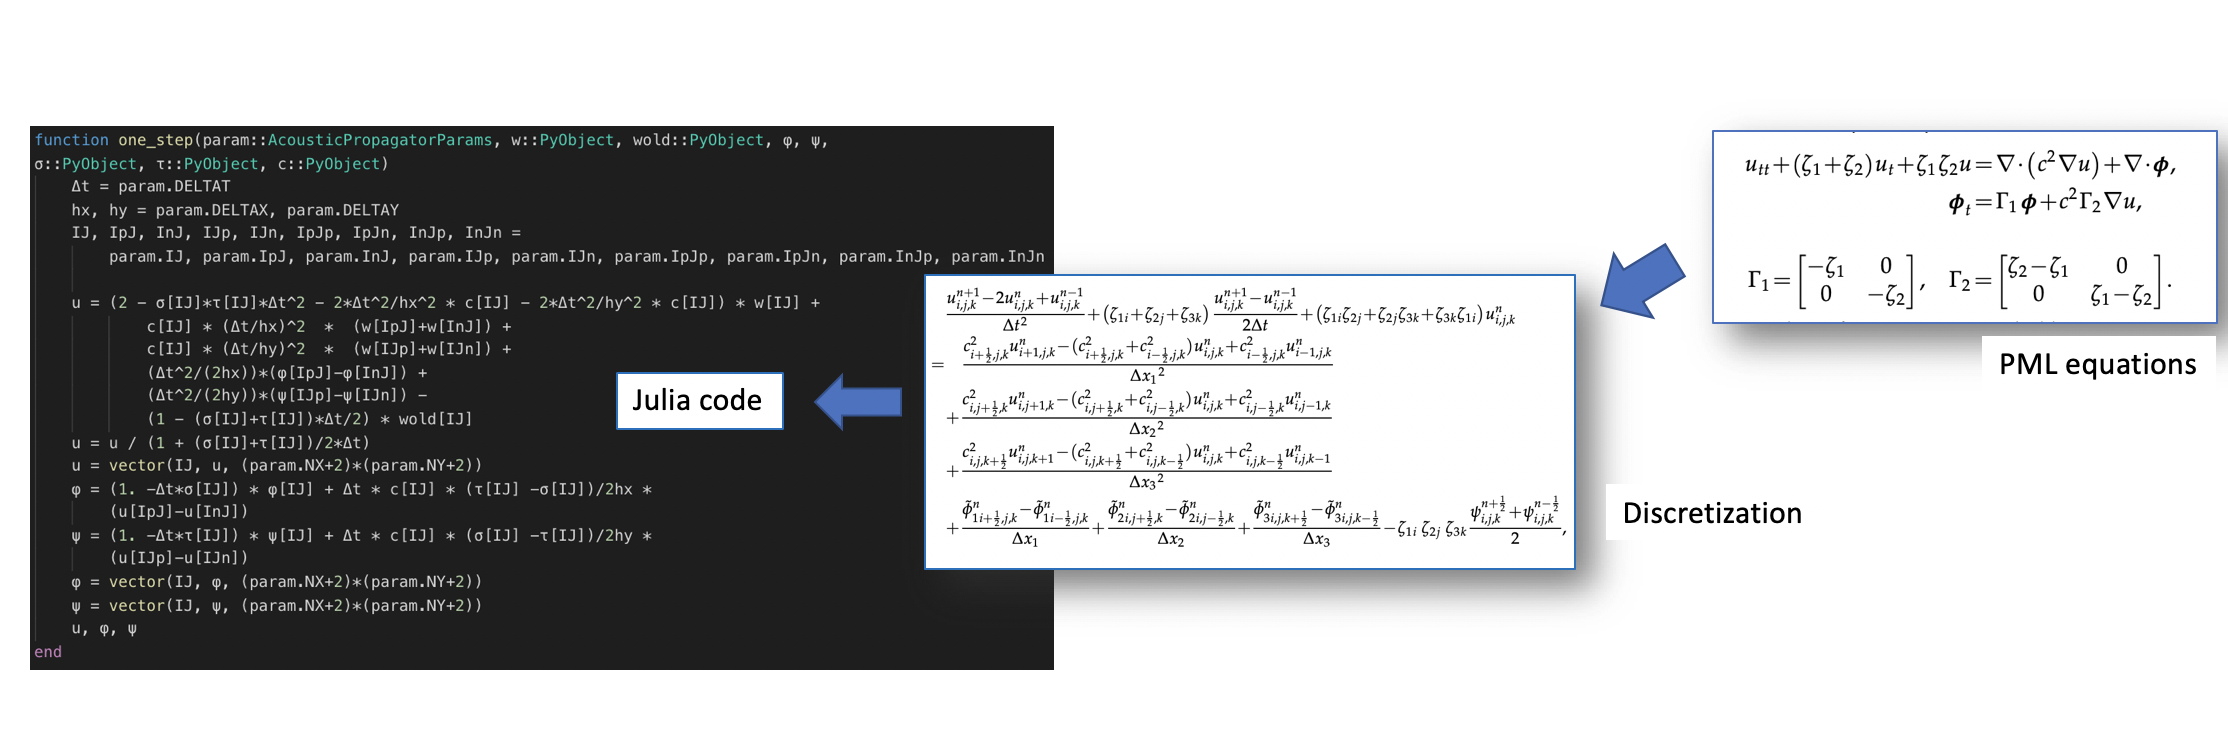
\includegraphics[width=1.0\textwidth]{../Julia.png}
\end{figure}
\end{frame}

%\begin{frame}
%	\frametitle{Code Example}
%	\begin{itemize}
%		\item  Find $b$ such that $u(0.5)=1.0$ and
%		$$-bu''(x)+u(x) = 8 + 4x - 4x^2, x\in[0,1], u(0)=u(1)=0$$
%	\end{itemize}
%	\begin{figure}[hbt]
%  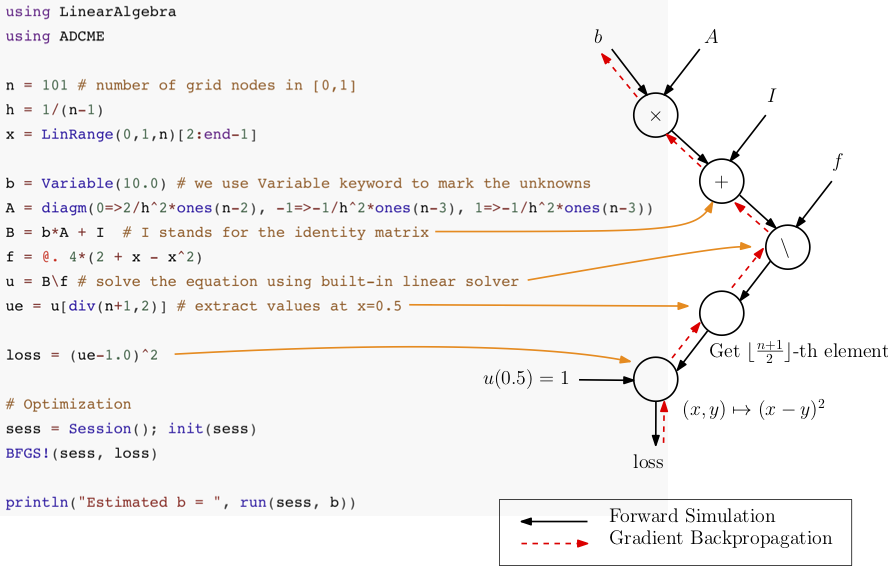
\includegraphics[width=0.8\textwidth]{../code.png}
%\end{figure}
%\end{frame}



\begin{frame}
	\frametitle{ADSeismic.jl: A General Approach to Seismic Inversion}
	\begin{itemize}
		\item Many seismic inversion problems can be solved within a unified framework. 
	\end{itemize}
	\begin{figure}[hbt]
  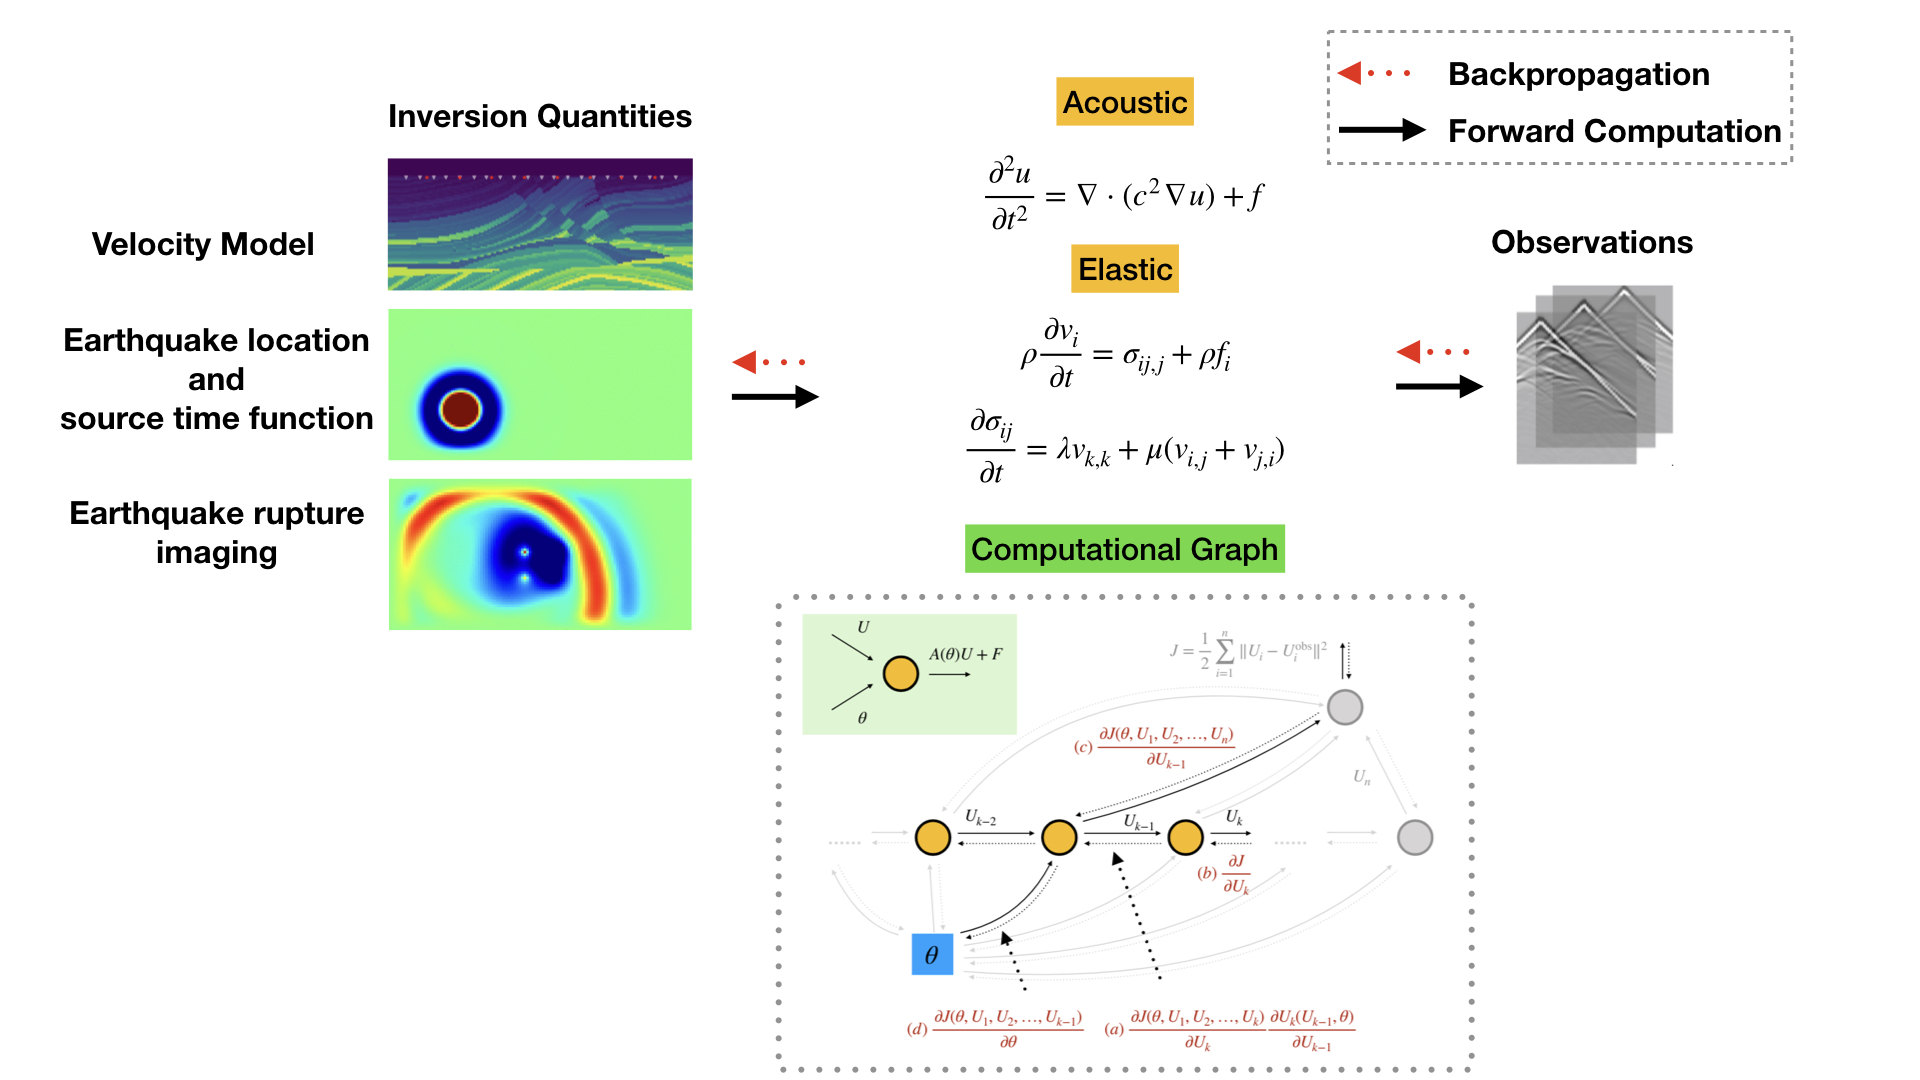
\includegraphics[width=1.0\textwidth]{../adseimic.jpeg}
\end{figure}
	
\end{frame}

\begin{frame}
	\frametitle{ADSeismic.jl: Earthquake Location Example}
	\begin{itemize}
		\item The earthquake source function is parameterized by ($g(t)$ and $x_0$ are unknowns)
		$$f(x, t) =  \frac{g(t)}{2\pi \sigma^2} \exp \left( -\frac{||x - x_0||^2}{2 \sigma^2} \right)$$
	\end{itemize}
	\begin{figure}[hbt]
  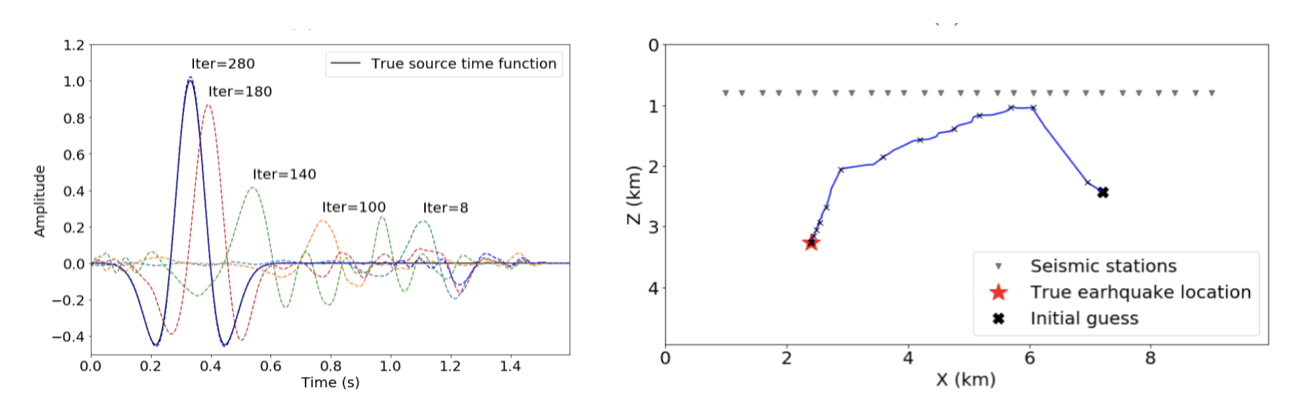
\includegraphics[width=1.0\textwidth]{../source_time}
\end{figure}
\end{frame}


\begin{frame}
	\frametitle{ADSeismic.jl: Benchmark}
	\begin{itemize}
		\item ADCME makes the heterogeneous computation capability of TensorFlow available for scientific computing. 
	\end{itemize}
	\begin{figure}[hbt]
  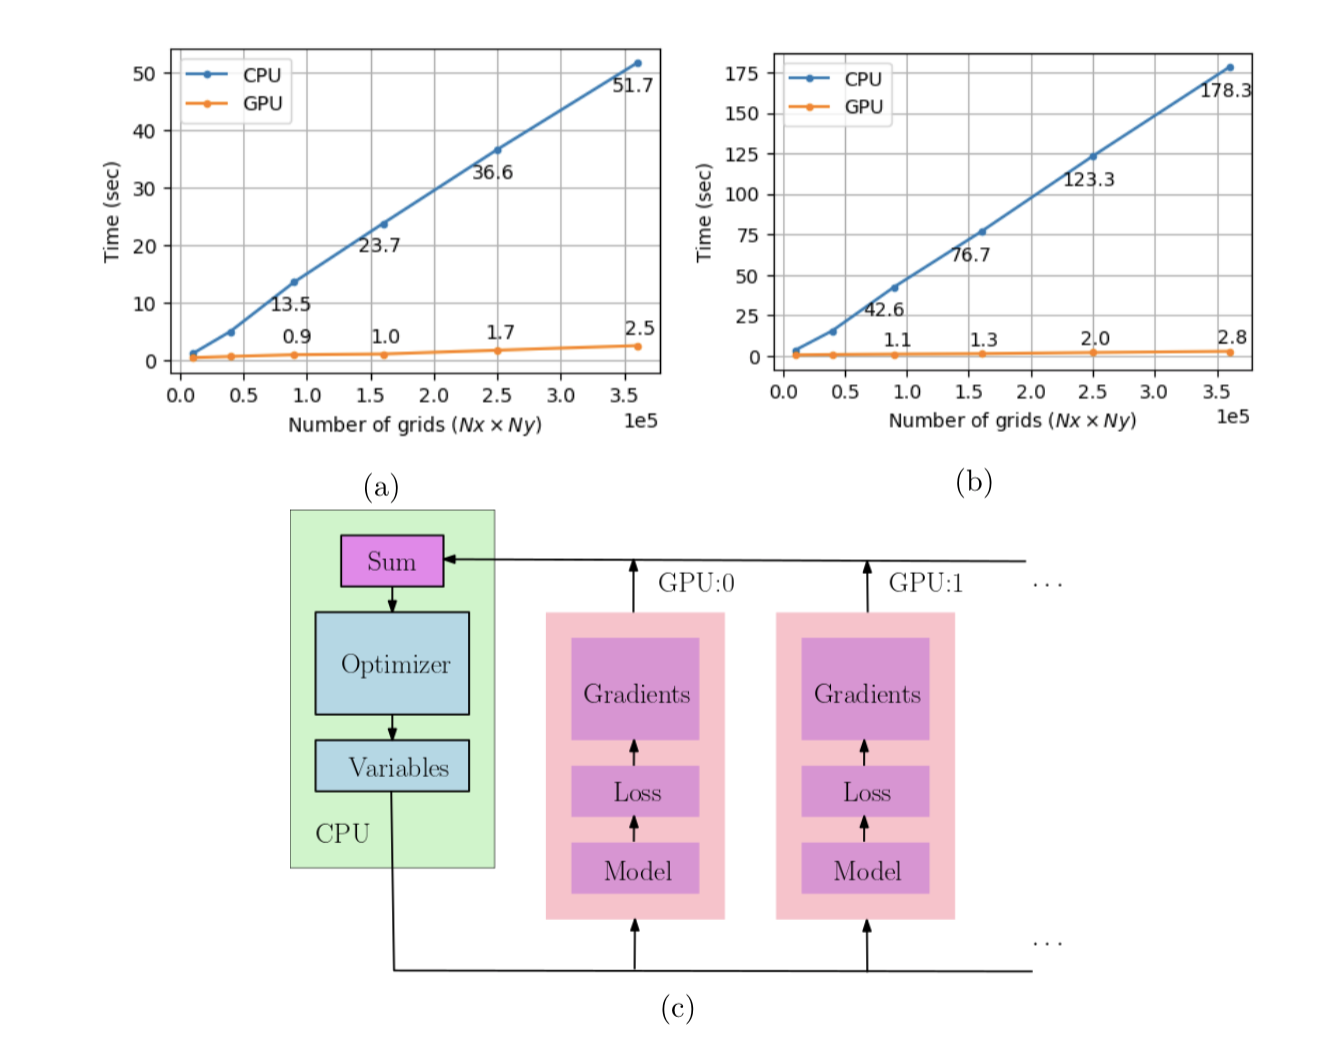
\includegraphics[width=0.7\textwidth]{../benchmark}
\end{figure}
\end{frame}

\begin{frame}
	\frametitle{NNFEM.jl: Constitutive Modeling}
	
	\begin{equation}\label{equ:momentum}
  \begin{aligned}
		\underbrace{\sigma_{ij,j}}_{\mbox{stress}} + \rho \underbrace{b_i}_{\mbox{external force}} &= \rho \underbrace{\ddot u_i}_{\mbox{velocity}}\\
		\underbrace{\varepsilon_{ij}}_{\mbox{strain}} &= \frac{1}{2}(u_{j,i}+u_{i,j})
	\end{aligned}
\end{equation}

	
	\begin{itemize}
		\item \textbf{Observable}: external/body force $b_i$, displacements $u_i$ (strains $\varepsilon_{ij}$ can be computed from $u_i$); density $\rho$ is known.  
		\item \textbf{Unobservable}: stress $\sigma_{ij}$. 
		\item Data-driven Constitutive Relations: modeling the strain-stress relation using a neural network
\begin{equation}\label{equ:nn}
  	\boxed{\mbox{stress} =\mathcal{M}_{\theta}(\mbox{strain},\ldots)}
\end{equation}
		and the neural network is trained by coupling (1) and (2).
	\end{itemize}


\end{frame}

\begin{frame}
	\frametitle{NNFEM.jl: Robustic Constitutive Modeling}
	\begin{itemize}
\item Proper form of constitutive relation is crucial for numerical stability
{\footnotesize\begin{align*}
 \mbox{Elasticity} &\Rightarrow \bm\sigma = \mathsf{C}_{\theta}\bm\epsilon \\
\mbox{Hyperelasticity } &\Rightarrow \begin{cases}\bm\sigma =\mathcal{M}_{\theta}(\bm\epsilon) & \mbox{(Static)} \\
\bm{\sigma}^{n+1}  =  \ChoL_{\bt}(\bm\epsilon^{n+1}) \ChoL_{\bt}(\bm\epsilon^{n+1})^T (\bm{\epsilon}^{n+1} - \bm{\epsilon}^{n})  + \bm{\sigma}^{n}  & \mbox{(Dynamic)} \end{cases} \\
	\mbox{Elaso-Plasticity} &\Rightarrow \bm\sigma^{n+1} = \ChoL_{\bt}(\bm\epsilon^{n+1},\bm{\epsilon}^{n},\bm{\sigma}^{n}) \ChoL_{\bt}(\bm\epsilon^{n+1},\bm{\epsilon}^{n},\bm{\sigma}^{n})^T (\bm{\epsilon}^{n+1} - \bm{\epsilon}^{n})  + \bm{\sigma}^{n} 
\end{align*}
}{\footnotesize$$\ChoL_{\bt} = \begin{bmatrix}
L_{1111}  &  & &  &       &\\
L_{2211}  & L_{2222} & &   & &\\
 L_{3311}  &  L_{3322}               & L_{3333} &  & &\\
               &                 &                 & L_{2323}&  &\\
              &               &                  &                & L_{1313} &\\
              &                 &                  &                &                 &L_{1212}\\
\end{bmatrix}$$}
	\item \textcolor{red}{Weak convexity}: $\ChoL_{\bt}\ChoL_{\bt}^T \succ 0$
	\item \textcolor{red}{Time consistency}:  $\bm\sigma^{n+1} \rightarrow \bm \sigma^n$ when $\bm\epsilon^{n+1} \rightarrow \bm \epsilon^n$
\end{itemize}

\end{frame}

\begin{frame}
	\frametitle{NNFEM.jl: Robustic Constitutive Modeling}
	\begin{itemize}
	 \item Weak form of balance equations of linear momentum 
	{\footnotesize
	\begin{align*}
		P_i(\theta) &= \int_V \rho \ddot u_i \delta u_i dVt + \int_{V} \textcolor{blue}{\underbrace{\textcolor{blue}{\sigma_{ij}(\theta)}}_{\mathclap{\textcolor{blue}{\mbox{embedded neural network}}}}} \delta \varepsilon_{ij}dV\\
		F_i &= \int_{V}\rho b_i \delta u_i dV + \int_{\partial V} t_i\delta u_idS
	\end{align*}
	}
	\item Train the neural network by 
	{\scriptsize $$\boxed{L(\theta) = \min_{\theta}\;\sum_{i=1}^N(P_i(\theta) - F_i)^2}$$}
	The gradient $\nabla L(\theta)$ is computed via automatic differentiation.
	\end{itemize}
	\begin{figure}[hbt]
  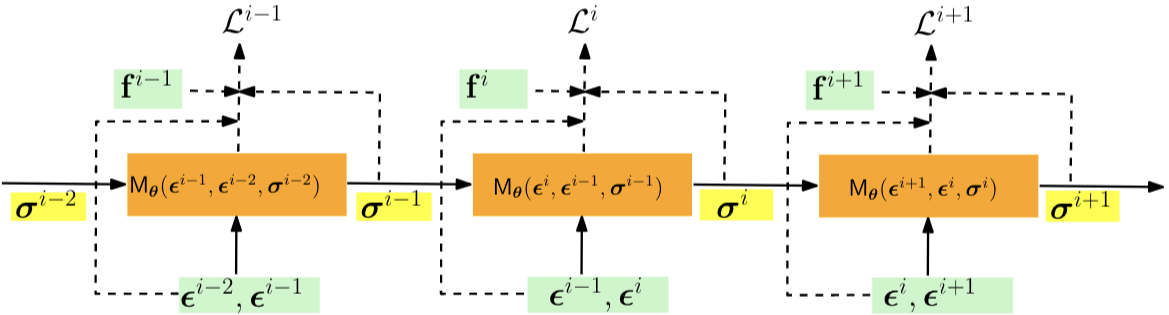
\includegraphics[width=0.75\textwidth]{../rnn}
\end{figure}

\end{frame}

\begin{frame}
	\frametitle{NNFEM.jl: Robustic Constitutive Modeling}
\begin{figure}[hbt]
  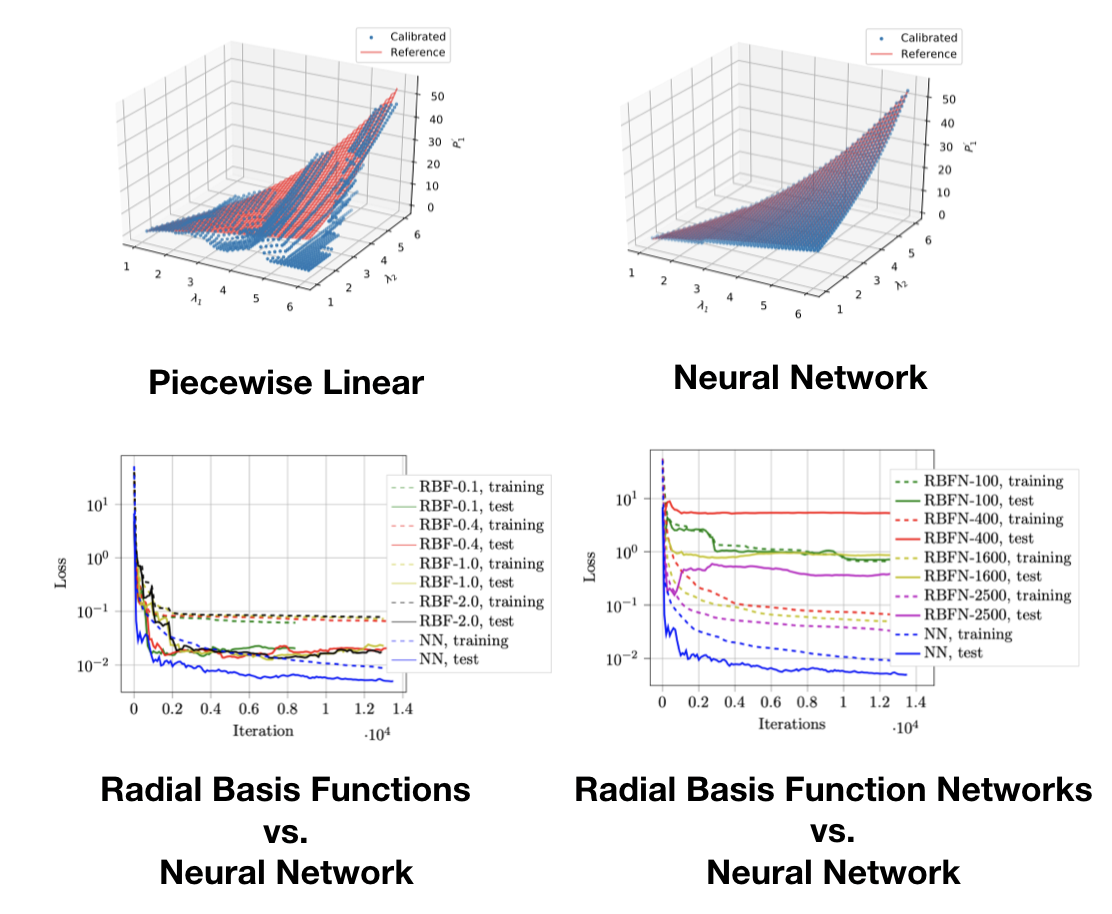
\includegraphics[width=0.8\textwidth]{../vs}
\end{figure}
\end{frame}


\begin{frame}
	\frametitle{NNFEM.jl: Robustic Constitutive Modeling}
	\begin{itemize}
		\item Comparison of different neural network architectures 
		\begin{align*}
			\bm\sigma^{n+1} &= \ChoL_{\bt}(\bm\epsilon^{n+1},\bm{\epsilon}^{n},\bm{\sigma}^{n}) \ChoL_{\bt}(\bm\epsilon^{n+1},\bm{\epsilon}^{n},\bm{\sigma}^{n})^T (\bm{\epsilon}^{n+1} - \bm{\epsilon}^{n})  + \bm{\sigma}^{n} \\
			\bm{\sigma}^{n+1} &=  \mathsf{NN}_{\bt}(\bm\epsilon^{n+1},\bm{\epsilon}^{n},\bm{\sigma}^{n})\\
			\bm{\sigma}^{n+1} &=  \mathsf{NN}_{\bt}(\bm\epsilon^{n+1},\bm{\epsilon}^{n},\bm{\sigma}^{n}) + \bm{\sigma}^{n}
		\end{align*}
	\end{itemize}
\begin{figure}[hbt]
  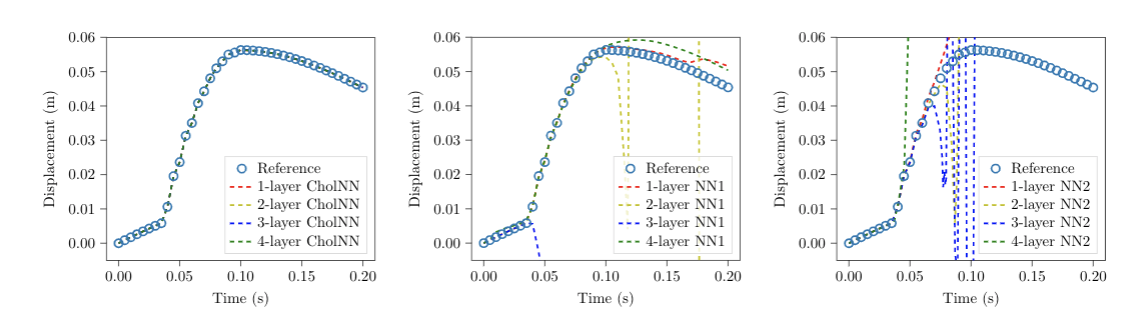
\includegraphics[width=1.0\textwidth]{../nncons}
\end{figure}
\end{frame}

\section{Beyond Automatic Differentiation: Physics Constrained Learning}
\begin{frame}


	\frametitle{Challenges in AD}
	
	
	\begin{minipage}[t]{0.49\textwidth}
	\vspace{-3cm}
\begin{itemize}
	\item Most AD frameworks only deal with explicit operators, i.e., the operators that can be expressed by differentiable library functions. 
	\item A large portion of scientific computing algorithms involve implicit schemes or iterative procedures to some extent.
\end{itemize}
\end{minipage}~
\begin{minipage}[t]{0.49\textwidth}
  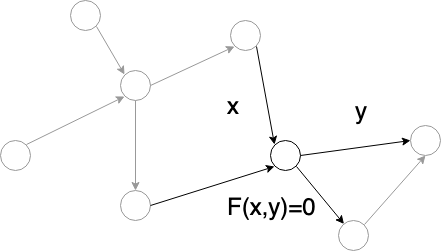
\includegraphics[width=1.0\textwidth]{../sim.png}
\end{minipage}

	% Please add the following required packages to your document preamble:
% \usepackage{booktabs}
\begin{table}[]
\begin{tabular}{@{}lll@{}}
\toprule
Linear/Nonlinear & Explicit/Implicit & Expression   \\ \midrule
Linear           & Explicit          & $y=Ax$       \\
Nonlinear        & Explicit          & $y = F(x)$   \\
\textbf{Linear}           & \textbf{Implicit}          & $Ax = y$     \\
\textbf{Nonlinear}        & \textbf{Implicit}          & $F(x,y) = 0$ \\ \bottomrule
\end{tabular}
\end{table}
\end{frame}

\begin{frame}
	\frametitle{Physics Constrained Learning}
	\begin{itemize}
		\item Let $L_h$ be a error functional, $F_h$ be the corresponding nonlinear implicit operator, $\theta$ be all the input to this operator and $u_h$ be all the output of this node.
 $${\small    \min_{\theta}\; L_h(u_h) \quad \mathrm{s.t.}\;\; F_h(\theta, u_h) = 0}$$

\item Assume in the forward computation, we solve for $u_h=G_h(\theta)$ in $F_h(\theta, u_h)=0$, and then
$${\small\tilde L_h(\theta)  = L_h(G_h(\theta))}$$
\item Applying the \textcolor{red}{implicit function theorem}
{  \scriptsize
\begin{equation*}
\frac{{\partial {F_h(\theta, u_h)}}}{{\partial \theta }} + {\frac{{\partial {F_h(\theta, u_h)}}}{{\partial {u_h}}}}  \frac{\partial G_h(\theta)}{\partial \theta} = 0  \Rightarrow 
     \frac{\partial G_h(\theta)}{\partial \theta} =  -\Big( \frac{{\partial {F_h(\theta, u_h)}}}{{\partial {u_h}}} \Big)^{ - 1} \frac{{\partial {F_h(\theta, u_h)}}}{{\partial \theta }}
\end{equation*}
}
\item Finally we have
{\scriptsize
\begin{equation*}
    \boxed{\frac{{\partial {{\tilde L}_h}(\theta )}}{{\partial \theta }} 
    = \frac{\partial {{ L}_h}(u_h )}{\partial u_h}\frac{\partial G_h(\theta)}{\partial \theta}= - \frac{{\partial {L_h}({u_h})}}{{\partial {u_h}}} \;
    \Big( {\frac{{\partial {F_h(\theta, u_h)}}}{{\partial {u_h}}}\Big|_{u_h = {G_h}(\theta )}} \Big)^{ - 1} \;
    \frac{{\partial {F_h(\theta, u_h)}}}{{\partial \theta }}\Big|_{u_h = {G_h}(\theta )}}
\end{equation*}
}

	\end{itemize}
	
\end{frame}


\begin{frame}
	\frametitle{Physics Constrained Learning}	
	{\scriptsize$$\boxed{\frac{{\partial {{\tilde L}_h}(\theta )}}{{\partial \theta }} 
    = - \frac{{\partial {L_h}({u_h})}}{{\partial {u_h}}} \;
    \Big( {\frac{{\partial {F_h(\theta, u_h)}}}{{\partial {u_h}}}\Big|_{u_h = {G_h}(\theta )}} \Big)^{ - 1} \;
    \frac{{\partial {F_h(\theta, u_h)}}}{{\partial \theta }}\Big|_{u_h = {G_h}(\theta )}}$$}
	\begin{minipage}[t]{0.48\textwidth}
		Step 1: Calculate $w$ by solving a linear system (never invert the matrix!)
{\scriptsize$$w^T = \underbrace{\frac{{\partial {L_h}({u_h})}}{{\partial {u_h}}\rule[-9pt]{1pt}{0pt}}}_{1\times N} 
        \;\;
        \underbrace{\Big( {\frac{{\partial {F_h}}}{{\partial {u_h}}}\Big|_{u_h = {G_h}(\theta )}} \Big)^{ - 1}}_{N\times N}$$}
Step 2: Calculate the gradient by automatic differentiation 
{\scriptsize$$w^T\;\underbrace{\frac{{\partial {F_h}}}{{\partial \theta }}\Big|_{u_h = {G_h}(\theta )}}_{N\times p} = \frac{\partial (w^T\;  {F_h}(\theta, u_h))}{\partial \theta }\Bigg|_{u_h = {G_h}(\theta )}$$}
	\end{minipage}\hfill\vline\hfill~
	\begin{minipage}[t]{0.48\textwidth}
		Step 1: Calculate $z$ by solving a linear system (never invert the matrix!)
		{\scriptsize$$z = \underbrace{
            \Big( {\frac{{\partial {F_h}}}{{\partial {u_h}}}\Big|_{u_h = {G_h}(\theta )}} \Big)^{ - 1}}_{N\times N}
            \;\; \underbrace{\frac{{\partial {F_h}}}{{\partial \theta }}\Big|_{u_h = {G_h}(\theta )}}_{N\times p}$$}
           Step 2: Calculate the gradient
           {\scriptsize$$\underbrace{\frac{{\partial {L_h}({u_h})}}{{\partial {u_h}}}}_{1\times N}\; z$$}
	\end{minipage}
	\begin{center}
		\textbf{Which strategy should we use?}
	\end{center}
\end{frame}

\begin{frame}
	\frametitle{Physics Constrained Learning: Linear System}
	
	\begin{itemize}
		\item Many physical simulations require solving a linear system 
		$$F_h(\theta_1,\theta_2, u_h) = \theta_1 - A(\theta_2)u_h$$
		\item The backpropagation formula
		\begin{align*}
			p &:=\frac{\partial \tilde L_h(\theta_1, \theta_2)}{\partial \theta_1} = \frac{\partial L_h(u_h)}{\partial u_h}A(\theta_2)^{-1}\\
			q &:=\frac{\partial \tilde L_h(\theta_1, \theta_2)}{\partial \theta_2} = -\frac{\partial L_h(u_h)}{\partial u_h}A(\theta_2)^{-1} \frac{\partial A(\theta_2)}{\partial \theta_2}
		\end{align*}
		which is equivalent to 
		$$A^T p^T =\left( \frac{\partial  L_h(u_h)}{\partial u_h} \right)^T\quad q = -p\frac{\partial A(\theta_2)}{\partial \theta_2} $$
	\end{itemize}
	
\end{frame}

\begin{frame}
	\frametitle{FwiFlow.jl: Elastic Full Waveform Inversion for subsurface flow problems with intelligent automatic differentiation}
	\begin{figure}[hbt]
  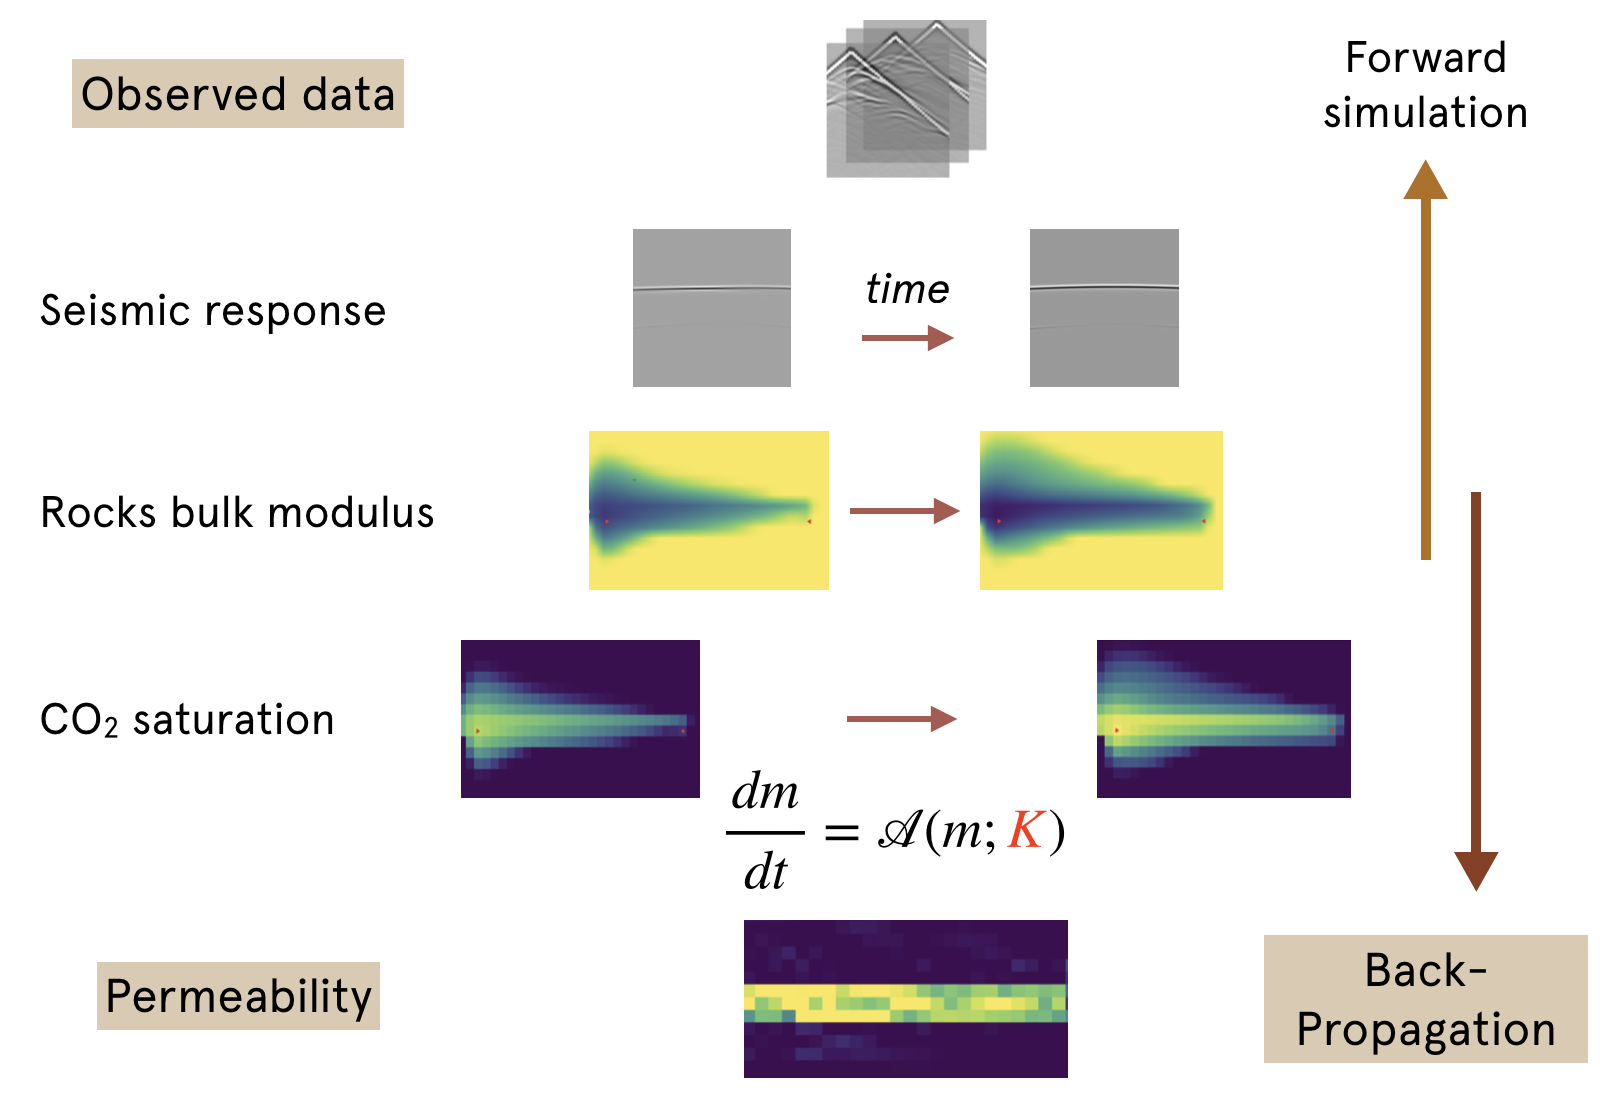
\includegraphics[width=0.8\textwidth]{../geo.png}
\end{figure}
\end{frame}

\begin{frame}
\frametitle{FwiFlow.jl: Fully Nonlinear Implicit Schemes}
\begin{itemize}
	\item The governing equation is a nonlinear PDE
{\scriptsize
	\begin{align*}
	\frac{\partial }{{\partial t}}(\phi {\textcolor{red}{S_i}}{\rho _i}) + \nabla  \cdot ({\rho _i}{\mathbf{v}_i}) &= {\rho _i}{q_i},\quad 
      i = 1,2	\\
      S_{1} + S_{2} &= 1\\
      {\mathbf{v}_i} &= - \frac{{K{\textcolor{red}{k_{ri}}}}}{{{\tilde{\mu}_i}}}(\nabla {P_i} - g{\rho _i}\nabla Z), \quad
      i=1, 2\\
	k_{r1}(S_1) =& \frac{k_{r1}^o S_1^{L_1}}{S_1^{L_1} + E_1 S_2^{T_1}}\\
	k_{r2}(S_1) =& \frac{ S_2^{L_2}}{S_2^{L_2} + E_2 S_1^{T_2}}
	\end{align*}
	}
	\item For stability and efficiency, implicit methods are the industrial standards. 
{\scriptsize	$$\phi (S_2^{n + 1} - S_2^n) - \nabla \cdot \left( {{m_{2}}(S_2^{n + 1})K\nabla \Psi _2^n} \right) \Delta t = 
\left(q_2^n + q_1^n \frac{m_2(S^{n+1}_2)}{m_1(S^{n+1}_2)}\right) 
\Delta t\quad m_i(s) = \frac{k_{ri}(s)}{\tilde \mu_i}
$$}
\item It is impossible to express the numerical scheme directly in an AD framework. Physics constrained learning is used to enhance the AD framework for computing gradients. 
\end{itemize}

\end{frame}

\begin{frame}
	\frametitle{FwiFlow.jl: Showcase}
	\begin{itemize}
		\item Task 1: Estimating the permeability from seismic data 
		\begin{figure}[hbt]
		\centering
  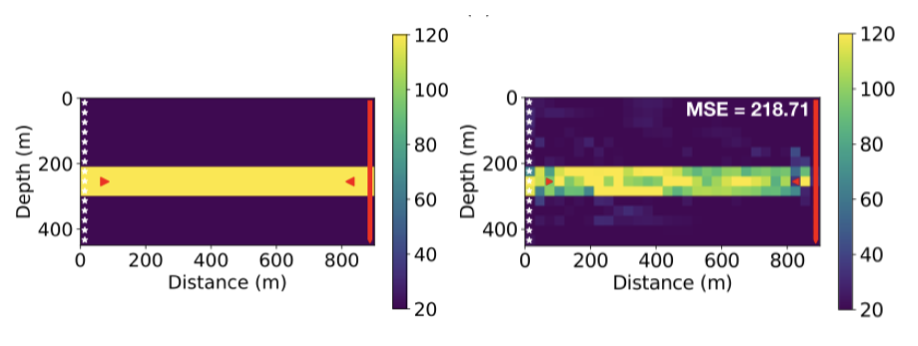
\includegraphics[width=0.6\textwidth]{../coupled}
\end{figure}
\item Task 2: Learning the rock physics model from sparse saturation data. The rock physics model is approximated by neural networks  
{\scriptsize$$f_1(S_1; \theta_1) \approx k_{r1}(S_1)\qquad f_2(S_1; \theta_2) \approx k_{r2}(S_1)$$}
\begin{figure}
	\centering
	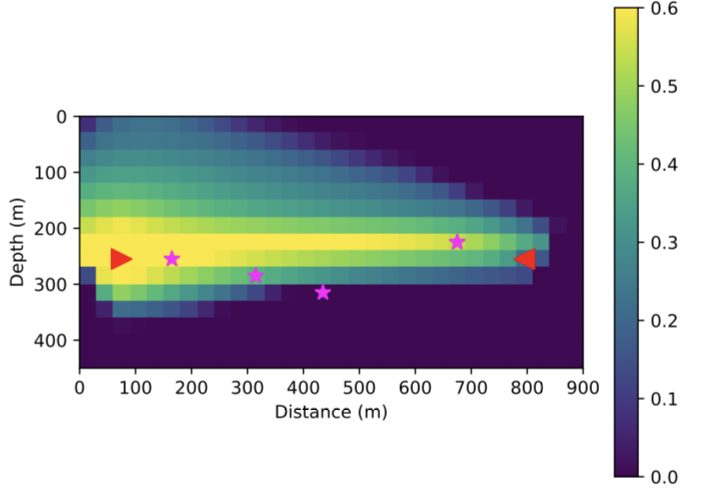
\includegraphics[width=0.25\textwidth]{../sat}~
  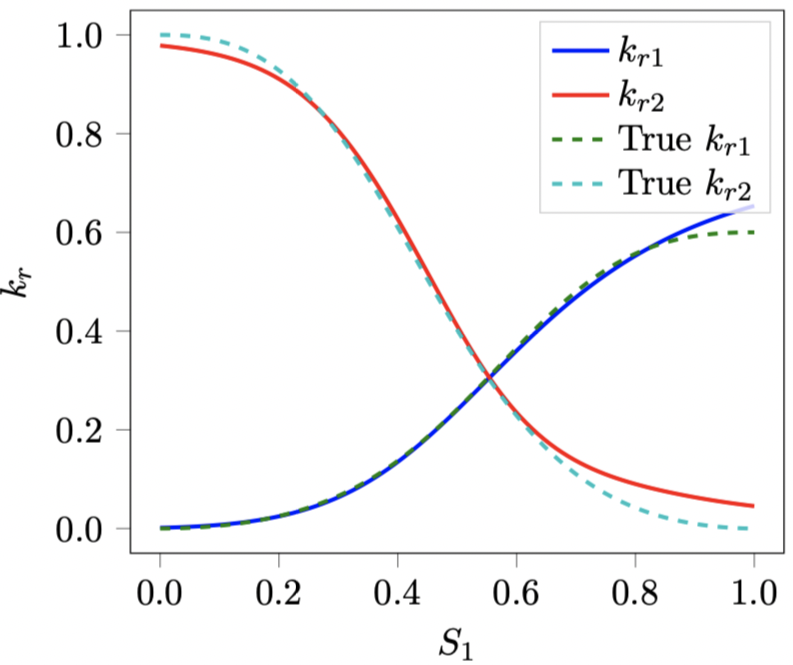
\includegraphics[width=0.25\textwidth]{../rock}
\end{figure}
	\end{itemize}
\end{frame}

\begin{frame}
	\frametitle{FwiFlow.jl: Showcase}
	\begin{itemize}
		\item Task 3: Learning the \textcolor{red}{nonlocal} (space or time) hidden dynamics from seismic data. This is very challenging using traditional methods (e.g., the adjoint-state method) because the dynamics is history dependent. 
	\end{itemize}
\begin{table}[htpb]
\centering
\begin{tabular}{@{}lll@{}}
\toprule
Governing Equation & $\sigma=0$ & $\sigma=5$ \\ \midrule
${}_0^CD_t^{\textbf{0.8}}m = 10\Delta m $ & \makecell{$a/a^*\ =1.0000$ \\  $\quad\alpha\quad =\mathbf{0.8000}$} & \makecell{$a/a^*\ =0.9109$ \\  $\quad\alpha\quad =\mathbf{0.7993}$} \\ \hline
${}_0^CD_t^{\textbf{0.2}}m = 10\Delta m $ & \makecell{$a/a^*\ =0.9994$ \\  $\quad\alpha\quad =\mathbf{0.2000}$} & \makecell{$a/a^*\ =0.3474$ \\  $\quad\alpha\quad =\mathbf{0.1826}$}  \\   \bottomrule
$\frac{\partial m}{\partial t} = -10(-\Delta)^{\textbf{0.2}} m$ & \makecell{$a/a^*\ =1.0000$ \\   $\quad s\quad =\mathbf{0.2000}$} & \makecell{$a/a^*\ =1.0378$ \\   $\quad s\quad =\mathbf{0.2069}$} \\  \hline
$\frac{\partial m}{\partial t} = -10(-\Delta)^{\textbf{0.8}} m$ & \makecell{$a/a^*\ =1.0000$ \\   $\quad s\quad =\mathbf{0.8000}$} & \makecell{$a/a^*\ =1.0365$ \\   $\quad s\quad =\mathbf{0.8093}$}\\  \bottomrule
\end{tabular}
\end{table}

\end{frame}


%\section{}
% Stochastic Inverse Problems 


\section{Some Perspectives}

\begin{frame}
	\frametitle{A Parameter/Function Learning View of Inverse Modeling}
	% Please add the following required packages to your document preamble:
% \usepackage{booktabs}
\begin{itemize}
	\item Most inverse modeling problems can be classified into 4 categories. To be more concrete, consider the PDE for describing physics
	\begin{equation}
		\nabla \cdot (\textcolor{red}{\theta} \nabla u(x)) = 0\quad \mathcal{B}\mathcal{C}(u(x)) = 0
	\end{equation}
	We observe some quantities depending on the solution $u$ and want to estimate $\theta$.
\end{itemize}
{
\tiny
\begin{table}[]
\begin{tabular}{@{}lllc@{}}
\toprule
Expression                                       & Description                & ADCME Solution                         & Note                                     \\ \midrule
$\nabla \cdot (\textcolor{red}{c} \nabla u(x)) = 0$ & Parameter Inverse Problem  & \makecell{Discrete Adjoint\\ State Method}          & \makecell{$c$ is the minimizer of\\ the error functional }                     \\ \hline
$\nabla \cdot (\textcolor{red}{f(x)} \nabla u(x)) = 0$ & Function Inverse Problem & \makecell{Neural Network \\ Functional Approximator} & $f(x) \approx f_{w}(x)$             \\ \hline
$\nabla \cdot (\textcolor{red}{f(u)} \nabla u(x)) = 0$ & Relation Inverse Problem   & \makecell{Residual Learning\\ Physics Constrained Learning}        & $f(u) \approx f_{w}(u)$             \\ \hline
$\nabla \cdot (\textcolor{red}{\varpi} \nabla u(x)) = 0$ & Stochastic Inverse Problem & \makecell{Generative Neural Networks}         & $\varpi = f_w(v_{\mathrm{latent}})$ \\ \bottomrule
\end{tabular}
\end{table}
}
\end{frame}

\begin{frame}
	\frametitle{Scopes, Challenges, and Future Work}
	\textcolor{red}{\textbf{Physics based machine learning}}: an innovative approach to inverse modeling. 
	{\scriptsize
	\begin{enumerate}
		\item Deep neural networks provide a novel function approximator that outperforms traditional basis functions in certain scenarios. 
		\item Numerical PDEs are not on the opposite side of machine learning. By expressing the known physical constraints using numerical schemes and approximating the unknown with machine learning models, we combine the best of the two worlds, leading to efficient and accurate inverse modeling tools. 
	\end{enumerate}
	}
		
		\textcolor{red}{\textbf{Automatic Differentiation}}: the core technique of physics based machine learning.
		{\scriptsize
		\begin{enumerate}
		\item The AD technique is not new; it has existed for several decades and many software exists. 
		\item The advent of deep learning drives the development of robust, scalable and flexible AD software that leverages the high performance computing environment. 
		\item As deep learning techniques continue to grow, crafting the tool to incorporate machine learning and AD techniques for inverse modeling is beneficial in scientific computing.
		\item However, AD is not a panacea. Many scientific computing algorithms cannot be directly expressed by composition of differentiable operators. 
	\end{enumerate}
	}
	
\end{frame}

\begin{frame}
	\frametitle{A General Approach to Inverse Modeling}
	\begin{figure}[hbt]
  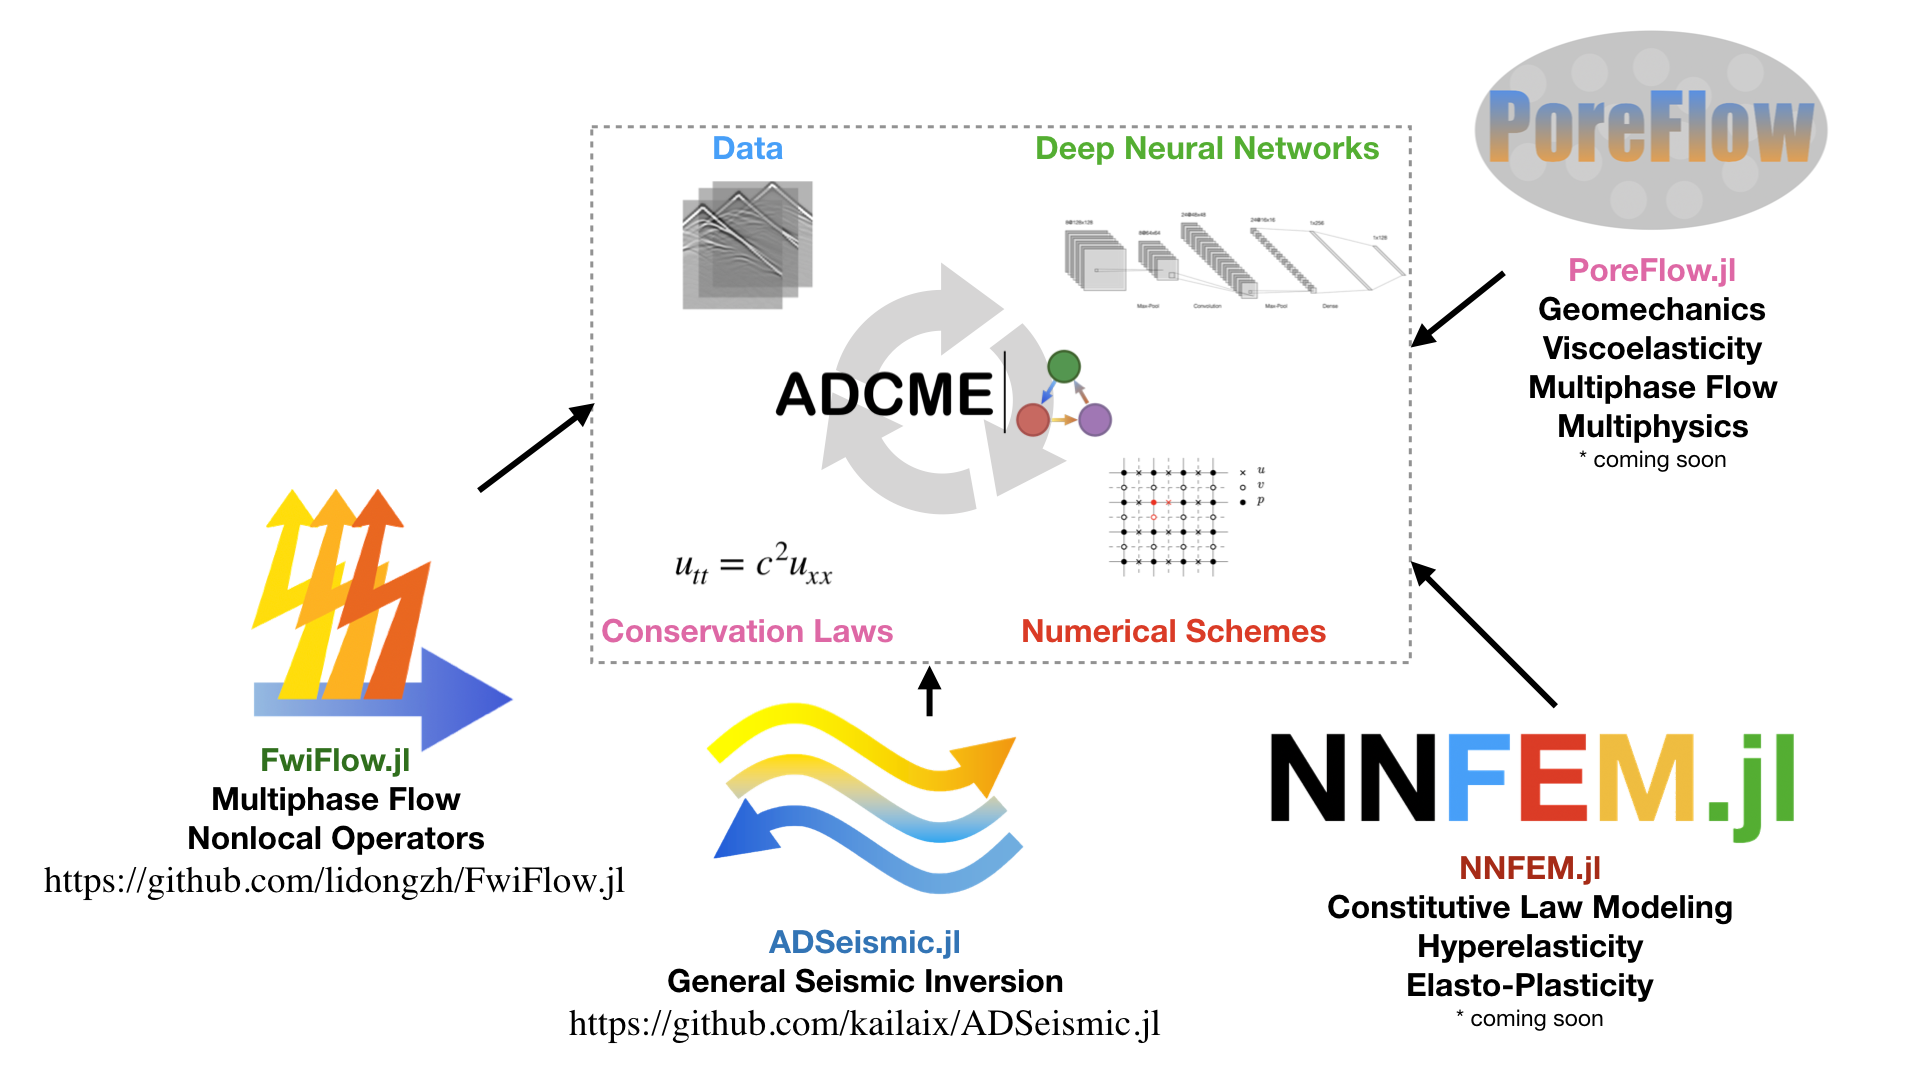
\includegraphics[width=1.0\textwidth]{../summary}
\end{figure}

\end{frame}

\begin{frame}
	\frametitle{Acknowledgement}
	\begin{itemize}
		\item \texttt{NNFEM.jl}: Joint work with Daniel Z. Huang and Charbel Farhat.
		\item \texttt{FwiFlow.jl}: Joint work with Dongzhuo Li and Jerry M. Harris. 
		\item \texttt{ADSeismic.jl}: Joint work with Weiqiang Zhu and Gregory C. Beroza. 
	\end{itemize}
\end{frame}


%}
%\usebackgroundtemplate{}
%----------------------------------------------------------------------------------------
%    PRESENTATION SLIDES
%----------------------------------------------------------------------------------------

%------------------------------------------------



\end{document} 